\PassOptionsToPackage{unicode=true}{hyperref} % options for packages loaded elsewhere
\PassOptionsToPackage{hyphens}{url}
%
\documentclass[12pt,twoside]{article}
\usepackage{lmodern}
\usepackage{amssymb,amsmath}
\usepackage{ifxetex,ifluatex}
\usepackage{fixltx2e} % provides \textsubscript
\ifnum 0\ifxetex 1\fi\ifluatex 1\fi=0 % if pdftex
  \usepackage[T1]{fontenc}
  \usepackage[utf8]{inputenc}
  \usepackage{textcomp} % provides euro and other symbols
\else % if luatex or xelatex
  \usepackage{unicode-math}
  \defaultfontfeatures{Ligatures=TeX,Scale=MatchLowercase}
\fi
% use upquote if available, for straight quotes in verbatim environments
\IfFileExists{upquote.sty}{\usepackage{upquote}}{}
% use microtype if available
\IfFileExists{microtype.sty}{%
\usepackage[]{microtype}
\UseMicrotypeSet[protrusion]{basicmath} % disable protrusion for tt fonts
}{}
\IfFileExists{parskip.sty}{%
\usepackage{parskip}
}{% else
\setlength{\parindent}{0pt}
\setlength{\parskip}{6pt plus 2pt minus 1pt}
}
\usepackage{hyperref}
\hypersetup{
            pdfborder={0 0 0},
            breaklinks=true}
\urlstyle{same}  % don't use monospace font for urls
\usepackage[margin=2.5cm]{geometry}
\usepackage{color}
\usepackage{fancyvrb}
\newcommand{\VerbBar}{|}
\newcommand{\VERB}{\Verb[commandchars=\\\{\}]}
\DefineVerbatimEnvironment{Highlighting}{Verbatim}{commandchars=\\\{\}}
% Add ',fontsize=\small' for more characters per line
\usepackage{framed}
\definecolor{shadecolor}{RGB}{248,248,248}
\newenvironment{Shaded}{\begin{snugshade}}{\end{snugshade}}
\newcommand{\AlertTok}[1]{\textcolor[rgb]{0.94,0.16,0.16}{#1}}
\newcommand{\AnnotationTok}[1]{\textcolor[rgb]{0.56,0.35,0.01}{\textbf{\textit{#1}}}}
\newcommand{\AttributeTok}[1]{\textcolor[rgb]{0.77,0.63,0.00}{#1}}
\newcommand{\BaseNTok}[1]{\textcolor[rgb]{0.00,0.00,0.81}{#1}}
\newcommand{\BuiltInTok}[1]{#1}
\newcommand{\CharTok}[1]{\textcolor[rgb]{0.31,0.60,0.02}{#1}}
\newcommand{\CommentTok}[1]{\textcolor[rgb]{0.56,0.35,0.01}{\textit{#1}}}
\newcommand{\CommentVarTok}[1]{\textcolor[rgb]{0.56,0.35,0.01}{\textbf{\textit{#1}}}}
\newcommand{\ConstantTok}[1]{\textcolor[rgb]{0.00,0.00,0.00}{#1}}
\newcommand{\ControlFlowTok}[1]{\textcolor[rgb]{0.13,0.29,0.53}{\textbf{#1}}}
\newcommand{\DataTypeTok}[1]{\textcolor[rgb]{0.13,0.29,0.53}{#1}}
\newcommand{\DecValTok}[1]{\textcolor[rgb]{0.00,0.00,0.81}{#1}}
\newcommand{\DocumentationTok}[1]{\textcolor[rgb]{0.56,0.35,0.01}{\textbf{\textit{#1}}}}
\newcommand{\ErrorTok}[1]{\textcolor[rgb]{0.64,0.00,0.00}{\textbf{#1}}}
\newcommand{\ExtensionTok}[1]{#1}
\newcommand{\FloatTok}[1]{\textcolor[rgb]{0.00,0.00,0.81}{#1}}
\newcommand{\FunctionTok}[1]{\textcolor[rgb]{0.00,0.00,0.00}{#1}}
\newcommand{\ImportTok}[1]{#1}
\newcommand{\InformationTok}[1]{\textcolor[rgb]{0.56,0.35,0.01}{\textbf{\textit{#1}}}}
\newcommand{\KeywordTok}[1]{\textcolor[rgb]{0.13,0.29,0.53}{\textbf{#1}}}
\newcommand{\NormalTok}[1]{#1}
\newcommand{\OperatorTok}[1]{\textcolor[rgb]{0.81,0.36,0.00}{\textbf{#1}}}
\newcommand{\OtherTok}[1]{\textcolor[rgb]{0.56,0.35,0.01}{#1}}
\newcommand{\PreprocessorTok}[1]{\textcolor[rgb]{0.56,0.35,0.01}{\textit{#1}}}
\newcommand{\RegionMarkerTok}[1]{#1}
\newcommand{\SpecialCharTok}[1]{\textcolor[rgb]{0.00,0.00,0.00}{#1}}
\newcommand{\SpecialStringTok}[1]{\textcolor[rgb]{0.31,0.60,0.02}{#1}}
\newcommand{\StringTok}[1]{\textcolor[rgb]{0.31,0.60,0.02}{#1}}
\newcommand{\VariableTok}[1]{\textcolor[rgb]{0.00,0.00,0.00}{#1}}
\newcommand{\VerbatimStringTok}[1]{\textcolor[rgb]{0.31,0.60,0.02}{#1}}
\newcommand{\WarningTok}[1]{\textcolor[rgb]{0.56,0.35,0.01}{\textbf{\textit{#1}}}}
\usepackage{graphicx,grffile}
\makeatletter
\def\maxwidth{\ifdim\Gin@nat@width>\linewidth\linewidth\else\Gin@nat@width\fi}
\def\maxheight{\ifdim\Gin@nat@height>\textheight\textheight\else\Gin@nat@height\fi}
\makeatother
% Scale images if necessary, so that they will not overflow the page
% margins by default, and it is still possible to overwrite the defaults
% using explicit options in \includegraphics[width, height, ...]{}
\setkeys{Gin}{width=\maxwidth,height=\maxheight,keepaspectratio}
\setlength{\emergencystretch}{3em}  % prevent overfull lines
\providecommand{\tightlist}{%
  \setlength{\itemsep}{0pt}\setlength{\parskip}{0pt}}
\setcounter{secnumdepth}{5}

% set default figure placement to htbp
\makeatletter
\def\fps@figure{htbp}
\makeatother

\usepackage{etoolbox}
\makeatletter
\providecommand{\subtitle}[1]{% add subtitle to \maketitle
  \apptocmd{\@title}{\par {\large #1 \par}}{}{}
}
\makeatother
% definição da linguagem
\usepackage[portuges]{babel}
%títulos da tabela em cima
\usepackage{floatrow}
\floatsetup[figure]{capposition=top}
\floatsetup[table]{capposition=top}

% Estilos do caption
\usepackage{caption}
\captionsetup[figure]{labelsep=period}
\captionsetup[table]{labelsep=period}

% cores dos links e ajustamento horizontal
\usepackage{hyperref}
\hypersetup{pdfstartview=FitH,colorlinks=true,linkcolor=black,urlcolor=blue,citecolor=blue,bookmarksopen,bookmarksdepth=3}

%cria o ambiente landscape
\usepackage{pdflscape}
\newcommand{\blandscape}{\begin{landscape}}
\newcommand{\elandscape}{\end{landscape}}

%identação do parágrafo
\setlength{\parindent}{0.7cm} % Default is 15pt.

% estilo das seções
\usepackage{titlesec}
\titleformat{\section}[block]
{\large\bfseries\centering}{\thesection.}{0.5em}{\MakeUppercase}{}

\titleformat{\subsection}[block]
{\normalfont\bfseries}{\thesubsection}{0.5em}{}

\titleformat{\subsubsection}[block]
{\normalfont\bfseries}{\thesubsubsection}{0.5em}{}

\titleformat{\subsubsubsection}[block]
{\normalfont\bfseries}{\thesubsubsubsection}{0.5em}{\newline}

% Pacote para cores
\usepackage[dvipsnames]{xcolor}

% Pacote para controlar estilo dos nomes dos autores
\usepackage{authblk}
\setlength{\affilsep}{.1em}

% estilo do header e do footer
\usepackage{fancyhdr}
\pagestyle{fancy}
\renewcommand{\sectionmark}[1]{\markright{\tiny #1}} 
\fancyhf{}
\makeatletter
  \fancyhead[RE]{\footnotesize{\sffamily\textcolor{darkgray}{\@title}}~~\normalsize{\thepage}}
\makeatother
\makeatletter
  \fancyhead[LO]{\normalsize{\thepage}~~\footnotesize{\sffamily\textcolor{darkgray}{\@title}}}
\makeatother
\rfoot{}
\renewcommand{\headrulewidth}{0pt}

% espaçemento da linha
\renewcommand{\baselinestretch}{1}

% altera a fonte
\usepackage[T1]{fontenc}
\usepackage{fbb}


% Alterando estilo do título
\makeatletter
\def\@maketitle{%
  \newpage
  \thispagestyle{empty}
  \null
  \vskip 1em%
  \begin{center}%
  \let \footnote \thanks
  {\Huge \@title \par}%
    \vskip 1.5em%
  %\begin{flushright}
  %\vskip 10em%
    {\large
      \lineskip .2em%
      %\sffamily \@author
      \@author}%
  %\end{flushright}
    \vskip 1em%
    %{\large \@date}%
  \end{center}%
  \par
  \vskip 1.5em}
\makeatother

% Muda estilo no sumário
%\usepackage{tocloft}
%\renewcommand{\cftsecfont}{\sffamily\bfseries}
%\renewcommand{\cftsubsecfont}{\sffamily}
%\renewcommand{\cftsubsubsecfont}{\sffamily}

% Ícones
\usepackage{fontawesome}

% título
\usepackage{titling}

% Informações do título
\setlength{\droptitle}{-2em}

  \title{Equilíbrio Geral Computável: Implementando o MINIMAL no R}
    \pretitle{\vspace{\droptitle}\centering\huge}
  \posttitle{\par}
    \author{Paulo Felipe Oliveira}
    \affil{\faGithub~paulofelipe}
    \preauthor{\centering\large\emph}
  \postauthor{\par}
      \predate{\centering\large\emph}
  \postdate{\par}
    \date{05/06/2019}

% tamanho da fonte dos códigos

\let\oldShaded\Shaded
\let\endoldShaded\endShaded
\renewenvironment{Shaded}{\footnotesize\oldShaded}{\endoldShaded}

%% change fontsize of output
\let\oldverbatim\verbatim
\let\endoldverbatim\endverbatim
\renewenvironment{verbatim}{\footnotesize\oldverbatim}{\endoldverbatim}

% Altear a espessura do bottomrule e toprule
\usepackage{booktabs}
\setlength\heavyrulewidth{0.1ex}
% https://github.com/rstudio/rmarkdown/issues/337
\let\rmarkdownfootnote\footnote%
\def\footnote{\protect\rmarkdownfootnote}

% https://github.com/rstudio/rmarkdown/pull/252
\usepackage{titling}
\setlength{\droptitle}{-2em}

\pretitle{\vspace{\droptitle}\centering\huge}
\posttitle{\par}

\preauthor{\centering\large\emph}
\postauthor{\par}

\predate{\centering\large\emph}
\postdate{\par}
\usepackage{booktabs}
\usepackage{longtable}
\usepackage{array}
\usepackage{multirow}
\usepackage{wrapfig}
\usepackage{float}
\usepackage{colortbl}
\usepackage{pdflscape}
\usepackage{tabu}
\usepackage{threeparttable}
\usepackage{threeparttablex}
\usepackage[normalem]{ulem}
\usepackage{makecell}
\usepackage{xcolor}
\usepackage[]{natbib}
\bibliographystyle{plainnat}

\date{}

\begin{document}

\maketitle

\begin{abstract}

zzzz

\noindent Este documento tem o objetivo de discutir a implementação de um modelo de equilíbrio geral simples no R usando o pacote `emr`. Como exemplo, utiliza-se o MINIMAL que é um modelo desenvolvido com propósitos educacionais pelos criadores do GEMPACK. Este modelo é de um único país com múltiplos setores, múltiplas fontes de demanda e comércio internacional. A definição dos modelos segue a abordagem descrita em \cite{zhang_2013}. Os resultados obtidos com o `emr` são consideravelmente próximos daqueles obtidos com o GEMPACK, ainda que aqui o modelo seja definido em variações relativas, diferentemente do GEMPACK que utiliza linearizações e métodos auxiliares para obter soluções mais exatas.
\end{abstract}

\hypertarget{introduuxe7uxe3o}{%
\section{Introdução}\label{introduuxe7uxe3o}}

Os modelos econômicos constituem uma ferramenta fundamental para o
desenvolvimento de análises por economistas. Para análises \emph{ex
ante}, tradicionalmente, são utilizados os modelos de equilíbrio parcial
ou de equilíbrio geral. Enquanto os modelos de equilíbrio parcial estão
focados em um mercado específico, os modelos de equilíbrio geral focam
na interação entre os diversos setores da economia. Conforme
\cite{burfisher2017}, o modelo de equilíbrio geral é economicamente
amplo porque considera as motivações e o comportamento de consumidores e
produtores e as suas ligações.

Apesar da microeconomia utilizada nos modelos tradicionais de equilíbrio
geral ser relativamente simples, a implementação de um modelo completo
pode ser uma tarefa não trivial. Para facilitar essa tarefa, duas
linguagens específicas foram desenvolvidas: GEMPACK e GAMS. É
incontestável que, muito provavelmente, especialistas em modelos de
equilíbrio geral irão trabalhar com uma dessas duas ferramentas.
Contudo, vale ressaltar que essas ferramentas necessitam da aquisição de
licenças para que seja possível trabalhar com modelos mais complexos em
termos do número de variáveis/equações.

O MINIMAL\footnote{\url{https://www.copsmodels.com/minimal.htm}}
(\cite{horridge_2001}) é um modelo de equilíbrio geral simplificado
utilizado em cursos introdutórios do GEMPACK. A partir desse modelo, é
possível deixar claro como a teoria microeconômica do consumidor e do
produtor podem ser combinadas para a construção de um modelo de
equilíbrio geral.

Este modelo considera 7 setores, um investidor agregado, um agente
representativo das famílias, exportações agregadas e o governo. Cada
produto pode ser obtido a partir de fontes domésticas ou importadas.

\hypertarget{estruturas-de-modelo-para-o-pacote-emr}{%
\section{Estruturas de Modelo para o Pacote
emr}\label{estruturas-de-modelo-para-o-pacote-emr}}

Para definirmos modelo com o pacote \texttt{emr} é preciso seguir uma
determinada estrutura para a definição de parâmetros, variáveis e
equações. No \texttt{emr}, é seguida a lógica descrita em
\cite{zhang_2013}. Conforme o referido autor, a crescente complexidade
dos modelos de equilíbrio geral torna-se uma barreira de entrada aos
potenciais novos analistas que desejam trabalhar com esse tipo de
ferramenta. \cite{zhang_2013} ressalta que o sistema de equações que
deve ser resolvido é desnecessariamente grande, uma vez que várias
equações e variáveis são acessórias.

Para ajudar a evitar esse problema, \cite{zhang_2013} define um sistema
de estruturação de modelos de equilíbrio geral. Nesse sistema, existem
apenas dois tipos de equações. O primeiro tipo define um conjunto de
variáveis que descrevem a teoria associada ao modelo. Por outro lado, o
segundo tipo de equações define condições de equilíbrio que devem ser
satisfeitas. Adicionalmente, cada tipo de equação está associado a um
tipo de variável, que chamaremos de definidas (\emph{defined}) e
não-definidas (\emph{undefined}). O sistema é resumido na Figura
\ref{system_structure}.

\begin{figure}[H]

{\centering 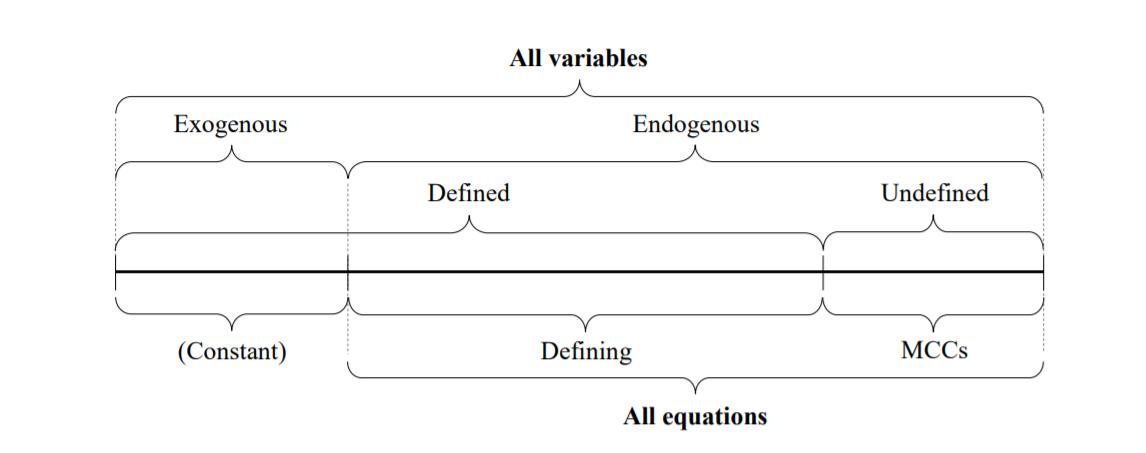
\includegraphics[width=5.73in]{structure_var_eq} 

}

\caption{Estrutura das variáveis e das equações (\cite{zhang_2013})\label{system_structure}}\label{fig:unnamed-chunk-1}
\end{figure}

Inicialmente, observa-se que, como usualmente é definido, as variáveis
podem ser exógenas ou endógenas. No entanto, é apresentada uma nova
classificação de variáveis: \emph{defined} e \emph{undefined}. As
variáveis definidas são aquelas que são constantes, definidas fora do
modelo, ou são definidas diretamente a partir dos valores das demais
variáveis. Por outro lado, as variáveis não-definidas não têm uma
equação que define o seu valor a partir das demais variáveis ou o seu
valor é definido de forma implícita, o que implica que é preciso
``chutar'' um valor inicial pra essa variável e depois checar se o valor
final da variável é igual ao chute inicial. Se não, o ``chute'' é
atualizado. As variáveis definidas são associadas com equações
definidoras (\emph{defining}) e as não-definidas são associadas às
equações de equilíbrio ``mcc'' (\emph{market clearing codition}).

No pacote \texttt{emr}, tem-se três funções principais que serão usadas
para criar as variáveis exógenas, as variáveis endógenas e as equações:

\begin{itemize}
\item
  \texttt{create\_param()}: cria parâmetros que são, no sentido amplo,
  as variáveis exógenas e outras constantes do modelo;
\item
  \texttt{create\_variable()}: cria variáveis (\emph{defined} e
  \emph{undefined}) para o modelo;
\item
  \texttt{create\_equation()}: cria as equações (\emph{defining} e
  \emph{mcc}) para o modelo.
\end{itemize}

Além dos parâmetros, das variáveis e das equações, o modelo também é
formado por outros componentes: \emph{sets} e equações de atualizações
(\emph{update equations}). Os \emph{sets} armazenam os índices de
variáveis e parâmetros. Por exemplo, suponha que \(X_i\) seja uma
variável e \(i\) possa assumir os valores {[}AGR, IND, SER{]}, assim
esse vetor de índices será chamado de \emph{set}. Por sua vez, as
equações de atualização servem para atualizar os valores iniciais de
alguns parâmetros a partir dos resultados da simulação. Por exemplo,
pode-se criar um parâmetro que guarde a informação da quantidade
consumida no dados iniciais, \(Q0\). Após a simulação, encontramos uma
variação na quantidade consumida. Essa variação pode ser utilizada para
atualizar o valor de \(Q0\) no novo equilíbrio.

Apesar do nosso foco ser em modelos de equilíbrio geral,vale a pena
introduzir o pacote com um modelo bastante simples de equilíbrio
parcial.

\hypertarget{exemplo-oferta-e-demanda}{%
\subsection{Exemplo: Oferta e Demanda}\label{exemplo-oferta-e-demanda}}

Aqui, vamos apresentar como um modelo pode ser construído e simulações
podem ser realizadas com o pacote \texttt{emr}. Para isso, iremos
trabalhar com o seguinte modelo:

\begin{itemize}
\tightlist
\item
  Curva de demanda: \[q^d = k^d [p (1 + t)]^{\eta}, \quad \eta < 0\]
\item
  Curva de oferta: \[q^s = k^s p^{\epsilon}, \quad \epsilon > 0\]
\item
  Equilíbrio de mercado: \[q^d = q^s\]
\end{itemize}

A Tabela \ref{oferta_demanda} detalha as variáveis e equações do modelo.
Nosso modelo tem 3 variáveis (\(q^d\), \(q^s\) e \(p\)) e três equações.
No entanto, perceba que as duas primeiras variáveis são definidas a
partir do preço \(p\). Dessa forma, o nosso ``sistema'' terá uma única
equação de equilíbrio e que estará associado a variável \(p\). Assim,
\(q^d\) e \(q^s\) são definidas e \(p\) é não definida.

\begin{table}[H]
\caption{Parâmetros e Variáveis do Modelo de Oferta e Demanda}\label{oferta_demanda}
\begin{tabular}{cccc}
\toprule
& Classe   & Tipo     & Descrição          \\
\hline
$q^d$ & Variável & Definida & Quantidade demanda \\
$q^s$ & Variável & Definida & Quantidade ofertada \\
$p$ & Variável & Não-definida & Preço \\
$t$ & Parâmetro & - & Imposto \\
$k^d$ & Parâmetro & - & Deslocamento da curva de demanda \\
$k^s$ & Parâmetro & - & Deslocamento da curva de oferta \\
\bottomrule
\multicolumn{4}{l}{Fonte: Elaboração própria.}\\
\end{tabular}
\end{table}

Também é interessante introduzir a lógica de escrita de modelos em
variações. Os modelos no GEMPACK são escritos em variações percentuais
obtidas a partir das linearizações das equações do modelo. No
\texttt{emr}, apesar de não ser obrigatório, em regra, iremos escrever o
modelo em variações relativas, a chamada \emph{exact-hat
algebra}\footnote{Na prática, reescrever as equações usando a
  \emph{exact-hat algebra} é similar a \emph{calibrated share form} que
  é usada em por alguns pesquisadores em CGE.} introduzida em
\cite{dekle_2008}.

A variação relativa de uma variável \(x\) entre dois equilíbrios é
denotada por \(\hat{x} = x^{\prime}/x\), em que \(x^\prime\) é o valor
de x no novo equilíbrio. A principal vantagem de utilizar o modelo em
variações é eliminar a necessidade de se obter os valores iniciais de
algumas variáveis e parâmetros. Por exemplo, uma constante desconhecida
\(k\), em variação, é reescrita como \(\hat{k} = 1\), uma vez que, a
priori, o seu valor é igual nos dois equilíbrios. Se os dados iniciais
representam um equilíbrio, o valor inicial da variáveis também será 1.

Reescrevendo o modelo de oferta e demanda em variações, temos as
seguintes equações:

\begin{itemize}
\tightlist
\item
  Curva de demanda:
  \[\hat{q}^d = \hat{k}^d [\hat{p}\hat{\tau}]^{\eta}, \quad \eta < 0\]
\item
  Curva de oferta:
  \[\hat{q}^s = \hat{k}^s \hat{p}^{\epsilon}, \quad \epsilon > 0\]
\item
  Equilíbrio de mercado: \[\hat{q}^d = \hat{q}^s\] Nessa formulação,
  \(\hat{\tau}\) é variação no poder do imposto, isto é:
  \[\hat{\tau} = \frac{1 + t^\prime}{1 + t}.\]
\end{itemize}

Antes de começar a implementar o modelo no R, precisamos dos dados base
que se referem a algum equilíbrio inicial. Usualmente, as bases de dados
para modelos de equilíbrio geral consideram apenas fluxos monetários. Na
prática, redefinindo-se a unidade de medida, assume-se preço inicial
igual a 1.

\begin{table}[H]
\caption{Dados Base para o Modelo de Oferta e Demanda}\label{dados_oferta_demanda}
\begin{tabular}{lc}
\toprule
Variável    & Valor\\
\hline
Valor inicial & 100 \\
Imposto inicial & 0\% \\
Elasticidade-preço da demanda ($\eta$) & -1 \\
Elasticidade-preço da oferta ($\epsilon$) & 0.5 \\
\bottomrule
Fonte: Elaboração própria. &  \\
\end{tabular}
\end{table}

Agora, vamos definir o modelo. Antes de mais nada, precisamos carregar o
pacote e inicializar alguns componentes do modelos:

\begin{Shaded}
\begin{Highlighting}[]
\KeywordTok{library}\NormalTok{(emr)}
\NormalTok{params <-}\StringTok{ }\KeywordTok{list}\NormalTok{()}
\NormalTok{variables <-}\StringTok{ }\KeywordTok{list}\NormalTok{()}
\NormalTok{equations <-}\StringTok{ }\KeywordTok{list}\NormalTok{()}
\end{Highlighting}
\end{Shaded}

Com o pacote carregado, iremos definir o bloco de demanda:

\begin{Shaded}
\begin{Highlighting}[]
\NormalTok{params[[}\StringTok{"K_d"}\NormalTok{]] <-}\StringTok{ }\KeywordTok{create_param}\NormalTok{(}
  \DataTypeTok{value =} \DecValTok{1}\NormalTok{,}
  \DataTypeTok{indexes =} \StringTok{"k_d"}\NormalTok{,}
  \DataTypeTok{desc =} \StringTok{"Shift na curva de demanda em variação"}
\NormalTok{)}

\NormalTok{params[[}\StringTok{"ETA"}\NormalTok{]] <-}\StringTok{ }\KeywordTok{create_param}\NormalTok{(}
  \DataTypeTok{value =} \FloatTok{-0.5}\NormalTok{,}
  \DataTypeTok{indexes =} \StringTok{"eta"}\NormalTok{,}
  \DataTypeTok{desc =} \StringTok{"Elasticidade-preço da demanda"}
\NormalTok{)}

\NormalTok{params[[}\StringTok{"TAU"}\NormalTok{]] <-}\StringTok{ }\KeywordTok{create_param}\NormalTok{(}
  \DataTypeTok{value =} \DecValTok{1}\NormalTok{,}
  \DataTypeTok{indexes =} \StringTok{"tau"}\NormalTok{,}
  \DataTypeTok{desc =} \StringTok{"Variação no poder do imposto"}
\NormalTok{)}

\CommentTok{# Vamos definir uma variável e uma equação}
\NormalTok{variables[[}\StringTok{"q_d"}\NormalTok{]] <-}\StringTok{ }\KeywordTok{create_variable}\NormalTok{(}
  \DataTypeTok{value =} \DecValTok{1}\NormalTok{,}
  \DataTypeTok{indexes =} \StringTok{"q_d"}\NormalTok{,}
  \DataTypeTok{type =} \StringTok{"defined"}\NormalTok{,}
  \DataTypeTok{desc =} \StringTok{"Variação na quantidade demandada"}
\NormalTok{)}

\NormalTok{equations[[}\StringTok{"E_q_d"}\NormalTok{]] <-}\StringTok{ }\KeywordTok{create_equation}\NormalTok{(}
  \StringTok{"q_d = K_d * (p * TAU)^ETA"}\NormalTok{,}
  \DataTypeTok{type =} \StringTok{"defining"}\NormalTok{,}
  \DataTypeTok{desc =} \StringTok{"Variação na quantidade demandada"}
\NormalTok{)}
\end{Highlighting}
\end{Shaded}

O segundo bloco é o da oferta:

\begin{Shaded}
\begin{Highlighting}[]
\NormalTok{params[[}\StringTok{"K_s"}\NormalTok{]] <-}\StringTok{ }\KeywordTok{create_param}\NormalTok{(}
  \DataTypeTok{value =} \DecValTok{1}\NormalTok{,}
  \DataTypeTok{indexes =} \StringTok{"k_s"}\NormalTok{,}
  \DataTypeTok{desc =} \StringTok{"Shift (em variação) na curva de oferta"}
\NormalTok{)}

\NormalTok{params[[}\StringTok{"EPS"}\NormalTok{]] <-}\StringTok{ }\KeywordTok{create_param}\NormalTok{(}
  \DataTypeTok{value =} \FloatTok{0.5}\NormalTok{,}
  \DataTypeTok{indexes =} \StringTok{"eta"}\NormalTok{,}
  \DataTypeTok{desc =} \StringTok{"Elasticidade-preço da oferta"}
\NormalTok{)}

\NormalTok{variables[[}\StringTok{"q_s"}\NormalTok{]] <-}\StringTok{ }\KeywordTok{create_variable}\NormalTok{(}
  \DataTypeTok{value =} \DecValTok{1}\NormalTok{,}
  \DataTypeTok{indexes =} \StringTok{"q_s"}\NormalTok{,}
  \DataTypeTok{type =} \StringTok{"defined"}\NormalTok{,}
  \DataTypeTok{desc =} \StringTok{"Variação na quantidade ofertada"}
\NormalTok{)}

\NormalTok{equations[[}\StringTok{"E_q_s"}\NormalTok{]] <-}\StringTok{ }\KeywordTok{create_equation}\NormalTok{(}
  \StringTok{"q_s = K_s * p^EPS"}\NormalTok{,}
  \DataTypeTok{type =} \StringTok{"defining"}\NormalTok{,}
  \DataTypeTok{desc =} \StringTok{"Variação na quantidade ofertada"}
\NormalTok{)}
\end{Highlighting}
\end{Shaded}

Para definição do preço de equilíbrio, utilizamos a equação de equilíbio
de mercado (\emph{mcc}). O único detalhe é que, ao invés de usarmos a
igualdade, iremos reescrevê-la de tal forma que o seu valor tenda a zero
quando o equilíbrio for encontrado. Isto é:

\[\hat{q}^d - \hat{q}^s\]

\begin{Shaded}
\begin{Highlighting}[]
\NormalTok{variables[[}\StringTok{"p"}\NormalTok{]] <-}\StringTok{ }\KeywordTok{create_variable}\NormalTok{(}
  \DataTypeTok{value =} \DecValTok{1}\NormalTok{,}
  \DataTypeTok{indexes =} \StringTok{"p"}\NormalTok{,}
  \DataTypeTok{type =} \StringTok{"undefined"}\NormalTok{,}
  \DataTypeTok{desc =} \StringTok{"Variação no preço"}
\NormalTok{)}

\NormalTok{equations[[}\StringTok{"E_p"}\NormalTok{]] <-}\StringTok{ }\KeywordTok{create_equation}\NormalTok{(}
  \StringTok{"q_d - q_s"}\NormalTok{,}
  \DataTypeTok{type =} \StringTok{"mcc"}\NormalTok{,}
  \DataTypeTok{desc =} \StringTok{"Equação de equilíbrio de mercado"}
\NormalTok{)}
\end{Highlighting}
\end{Shaded}

Apesar de não ser estritamente necessário, criaremos um parâmetro que
guardará o valor do equilíbrio inicial. Chamaremos de \(V^0\). No novo
equilíbrio, tem-se que
\[V^{0\prime} = V^0 \times \hat{p} \times \hat{q}^d.\] Utilizaremos as
equações de atualizações para atualizar esse valor:

\begin{Shaded}
\begin{Highlighting}[]
\NormalTok{params[[}\StringTok{"V0"}\NormalTok{]] <-}\StringTok{ }\KeywordTok{create_param}\NormalTok{(}
  \DataTypeTok{value =} \DecValTok{100}\NormalTok{,}
  \DataTypeTok{indexes =} \StringTok{"V0"}\NormalTok{,}
  \DataTypeTok{desc =} \StringTok{"Valor do equilíbrio inicial"}
\NormalTok{)}
\NormalTok{update_equations <-}\StringTok{ }\KeywordTok{list}\NormalTok{()}
\NormalTok{update_equations[[}\StringTok{"V0"}\NormalTok{]] <-}\StringTok{ }\KeywordTok{create_equation}\NormalTok{(}
  \StringTok{"V0 = V0 * p * q_d"}\NormalTok{,}
  \DataTypeTok{desc =} \StringTok{"Atualização do valor de equilíbrio"}
\NormalTok{)}
\end{Highlighting}
\end{Shaded}

Agora, vamos criar o objeto que conterá os elementos do modelo de oferta
e demanda. Este objeto deve ser uma lista nomeada como os
componentes\footnote{Os possíveis componentes são: sets, params,
  variables, equations e update\_equations}.

\begin{Shaded}
\begin{Highlighting}[]
\NormalTok{modelo_oferta_demanda <-}\StringTok{ }\KeywordTok{list}\NormalTok{(}
  \DataTypeTok{params =}\NormalTok{ params,}
  \DataTypeTok{variables =}\NormalTok{ variables,}
  \DataTypeTok{equations =}\NormalTok{ equations,}
  \DataTypeTok{update_equations =}\NormalTok{ update_equations}
\NormalTok{)}
\end{Highlighting}
\end{Shaded}

Adicionalmente, vamos testar se o modelo encontra-se em equilíbrio. Para
isso, iremos utilizar a função \texttt{solve\_emr()}\footnote{A função
  \texttt{solve\_emr()} utiliza o pacote BB desenvolvido por
  \cite{varadhan_gilbert_2009}. Também é fornecida a função
  \texttt{solve\_emr\_block()} que é baseada no método DF-SANE, porém em
  uma versão simplificada na qual o \emph{stepsize} e a atualização das
  variáveis são definidos equação a equação, além de possibilitar a
  utilização de um stepsize fixo para cada variável não-definida.}.

\begin{Shaded}
\begin{Highlighting}[]
\NormalTok{solucao <-}\StringTok{ }\KeywordTok{solve_emr}\NormalTok{(modelo_oferta_demanda)}
\CommentTok{# A função solve_emr retorna os seguintes elementos}
\KeywordTok{names}\NormalTok{(solucao)}
\end{Highlighting}
\end{Shaded}

\begin{verbatim}
## [1] "sol"                    "params"                 "variables"             
## [4] "updated_data"           "variables_descriptions" "params_descriptions"
\end{verbatim}

\begin{Shaded}
\begin{Highlighting}[]
\CommentTok{# o objeto sol apresenta os detalhes da solução}
\NormalTok{solucao}\OperatorTok{$}\NormalTok{sol}
\end{Highlighting}
\end{Shaded}

\begin{verbatim}
## $par
## p 
## 1 
## 
## $residual
## [1] 0
## 
## $fn.reduction
## [1] 0
## 
## $feval
## [1] 1
## 
## $iter
## [1] 0
## 
## $convergence
## [1] 0
## 
## $message
## [1] "Successful convergence"
## 
## $cpar
## method      M     NM 
##      2     50      0
\end{verbatim}

Com o modelo finalizado, vamos utilizá-lo para o que realmente
interessa: realizar simulações a partir de cenários. Como exemplo, vamos
supor que a tarifa inicial de 0\% foi alterada para 10\%. Qual é o novo
equilíbrio de mercado? O que aconteceria com a quantidade e com o preço?
Assim, iremos fazer \(\hat{\tau} = 1.1\). O seu valor inicial é igual 1.

\begin{Shaded}
\begin{Highlighting}[]
\NormalTok{modelo_oferta_demanda}\OperatorTok{$}\NormalTok{params}\OperatorTok{$}\NormalTok{TAU}\OperatorTok{$}\NormalTok{value}
\end{Highlighting}
\end{Shaded}

\begin{verbatim}
## tau 
##   1
\end{verbatim}

Para criar o choque, precisamos alterar o paramêmetro \texttt{TAU}.
Assim, basta modificar o seu valor para 1.1 (1.10/1). Note que chamamos
\texttt{value{[}{]}}, a chamada com \texttt{{[}{]}} garante que o nome
do elemento não seja sobrescrito.

\begin{Shaded}
\begin{Highlighting}[]
\NormalTok{modelo_oferta_demanda}\OperatorTok{$}\NormalTok{params}\OperatorTok{$}\NormalTok{TAU}\OperatorTok{$}\NormalTok{value[] <-}\StringTok{ }\FloatTok{1.1}
\end{Highlighting}
\end{Shaded}

Após a criação do choque, iremos resolver o modelo novamente. Os novos
valores das variáveis estarão no elemento \texttt{variables}. O novo
valor de equilíbrio, atualização de \(V^0\), está no elemento
\texttt{updated\_data}.

\begin{Shaded}
\begin{Highlighting}[]
\NormalTok{solucao_cen1 <-}\StringTok{ }\KeywordTok{solve_emr}\NormalTok{(modelo_oferta_demanda)}
\NormalTok{solucao_cen1}\OperatorTok{$}\NormalTok{variables}
\end{Highlighting}
\end{Shaded}

\begin{verbatim}
## $q_d
##       q_d 
## 0.9764541 
## 
## $q_s
##       q_s 
## 0.9764541 
## 
## $p
##         p 
## 0.9534625
\end{verbatim}

\begin{Shaded}
\begin{Highlighting}[]
\NormalTok{solucao_cen1}\OperatorTok{$}\NormalTok{updated_data}
\end{Highlighting}
\end{Shaded}

\begin{verbatim}
## $V0
##       V0 
## 93.10124
\end{verbatim}

O resultado para \texttt{q\_d} foi de 0.9765, o que indica que a nova
quantidade demandada é 2,4\% (\((0.9765 - 1) \times 100\)) menor do que
no equilíbrio inicial. A Tabela \ref{tab:resultados_oferta_demanda}
apresenta as variações para a quantidade, preço do produtor e preço do
consumidor. Verifica-se que o custo do imposto foi suportado, quase na
mesma proporção, pelos consumidores e produtores.

\begin{table}[!h]

\caption{\label{tab:resultados_oferta_demanda}Variações para um Choque de 10\% no Imposto}
\centering
\begin{tabular}[t]{c>{\raggedleft\arraybackslash}p{7em}}
\toprule
Variável & Variação\\
\midrule
$\hat{q}^d$ & -2,4\%\\
$\hat{p}$ & -4,7\%\\
$\hat{p}\hat{\tau}$ & 4,9\%\\
\bottomrule
\multicolumn{2}{l}{Fonte: Elaboração própria.}\\
\end{tabular}
\end{table}

Assim, concluímos o nosso primeiro exemplo. A lógica aplicada, em grande
parte, é a mesma que será utilizada em um modelo mais ``complexo'' de
equilíbrio geral. Começaremos, então, pelo MINIMAL.

\hypertarget{implementando-o-minimal-no-r}{%
\section{Implementando o MINIMAL no
R}\label{implementando-o-minimal-no-r}}

Nesta seção iremos implementar o MINIMAL, que recebe esse nome em razão
de ser uma versão em ``miniatura'' do modelo ORANI, desenvolvido por
\cite{horridge_2000}. Os dados para esse modelo podem ser obtidos nas
matrizes de insumo e produto disponibilizadas pelo órgãos oficiais de
estatísticas nacionais. Nesse documento, iremos utilizar a base de dados
para a Austrália. Primeiro trabalharemos os dados e depois iremos
implementar o modelo.

\hypertarget{dados-para-o-modelo}{%
\subsection{Dados para o Modelo}\label{dados-para-o-modelo}}

Os dados para o modelo são esquematizados conforme a Figura
\ref{model_database}. O esquema é similar ao de uma matriz de insumo
produto, na qual os elementos das linhas vendem para os elementos das
colunas.

\begin{figure}[h]

{\centering 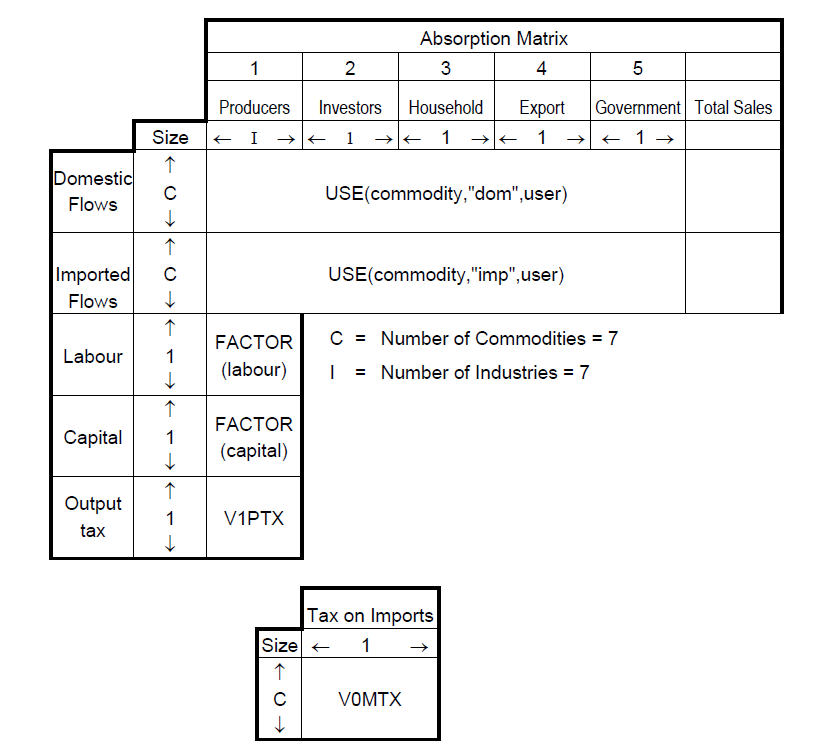
\includegraphics[width=5.55in]{minimal_database} 

}

\caption{Base de Dados para o Minimal(\cite{horridge_2001}\label{model_database})}\label{fig:unnamed-chunk-12}
\end{figure}

Fica claro na Figura \ref{model_database} que existem duas fontes
(\emph{sources}) de fornecimento de produtos: doméstica e importada.
Esse produtos são demandados pelos \(I\) setores produtores, pelos
investidores, pelas famílias, pelas exportações\footnote{O fornecimento
  de produtos importados para exportação é igual a zero.} e pelo
governo. As somas das linhas para produtos (\emph{commodities})
domésticos ou importados serão denominadas de vendas (\emph{sales}).
Note que a numeração das colunas serão utilizadas para identificar os
usuários. Por exemplo, 1 para indústrias e 3 para as famílias.

Adicionalmente, os fatores trabalhos e capital são demandados pelos
produtores, e há uma taxação sobre a produção. Por fim, independente do
demandante, existe um imposto de importação por produto. O valor
arrecadado de imposto de importação não é separado por usuário, o que
resulta em uma única taxa de importação por produto.

A tabela apresentada na Figura \ref{dados_australia} detalha um conjunto
de valores para a Austrália a partir de dados de 1986-1987. Os valores
estão a preços dos produtores. Ou seja, inclui qualquer imposto indireto
que possa ter sido aplicada àquele fluxo. Para cada setor produtor, a
sua produção (soma da respectiva coluna) tem que ser igual às suas
vendas (soma da respectiva linha). Por exemplo, a produção do setor
Agricultura-Mineração (AgricMining) foi igual 45.730, que é o mesmo
valor de suas vendas.

Para as importações de produtos manufaturados (\emph{Manufacture}), foi
recolhido o montante de 5.787. O valor total importado desses produtos
foi de 42.087 (este valor já inclui o imposto de importação), o que
implica em uma taxa de importação de 15,94\%\footnote{5787/(42087 -
  5787).}.

\begin{figure}

{\centering 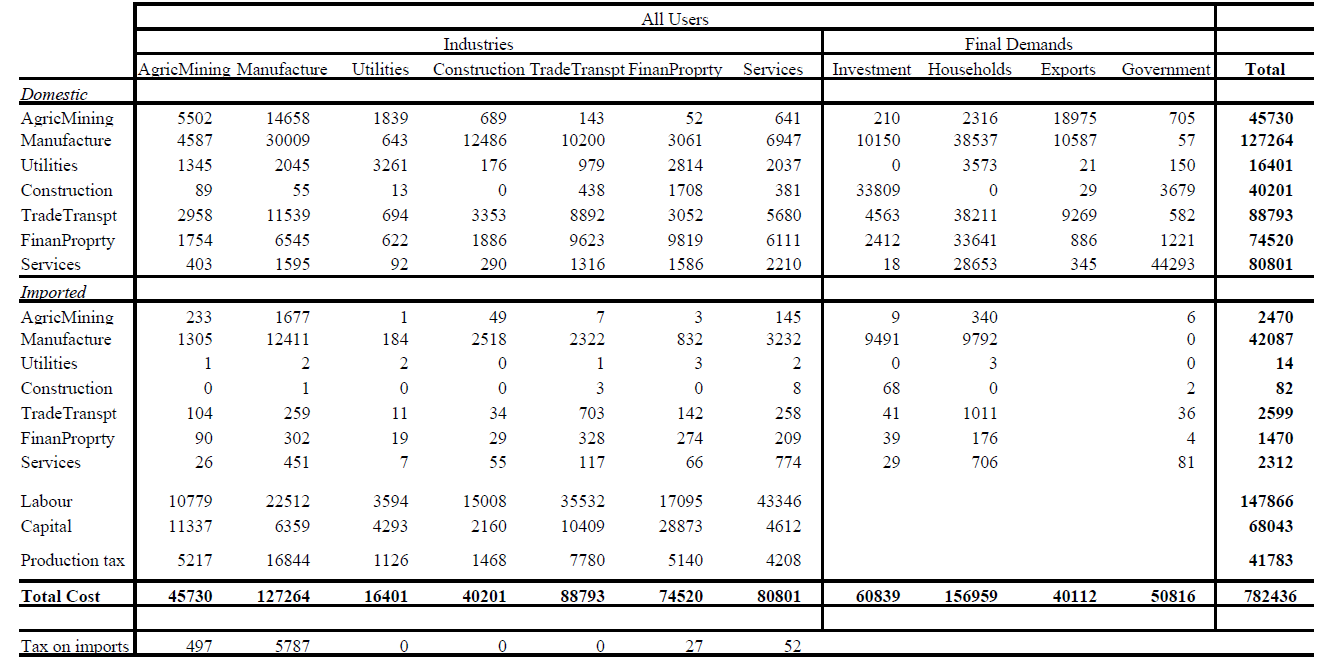
\includegraphics[width=8.83in,angle=90]{minimal_database_australia} 

}

\caption{Base de Dados para Austrália (Milhões 1986-1987)\label{dados_australia}}\label{fig:unnamed-chunk-13}
\end{figure}

\hypertarget{implementauxe7uxe3o}{%
\subsection{Implementação}\label{implementauxe7uxe3o}}

Nesta subseção, iremos detalhar a estrutura teórica do modelo e
implementá-lo no \texttt{R} com o pacote \texttt{emr}.

\hypertarget{passos-iniciais}{%
\subsubsection{Passos Iniciais}\label{passos-iniciais}}

Inicialmente, é preciso carregar o pacote \texttt{emr}:

\begin{Shaded}
\begin{Highlighting}[]
\KeywordTok{library}\NormalTok{(emr)}
\CommentTok{# Carregar o tidyverse para manipulação dos dados}
\KeywordTok{library}\NormalTok{(tidyverse)}
\end{Highlighting}
\end{Shaded}

Adicionalmente, também é necessário ler os dados que servirão de base
para o modelo. Os dados foram exportados do formato HAR do GEMPACK para
csv. Nessa conversão, as diversas tabelas são empilhadas em um único
csv, sendo separadas por uma linha denominada de \emph{HEADER}.

Dessa forma, vamos inicialmente identificar os \emph{headers}:

\begin{Shaded}
\begin{Highlighting}[]
\NormalTok{minimal_headers <-}\StringTok{ }\KeywordTok{read_lines}\NormalTok{(}\StringTok{'../dados/minimal.csv'}\NormalTok{)}

\NormalTok{minimal_headers[}\KeywordTok{str_detect}\NormalTok{(minimal_headers, }\StringTok{"Header"}\NormalTok{)]}
\end{Highlighting}
\end{Shaded}

\begin{verbatim}
## [1] "!Header: USE , dimensions: COM*SRC*USER [7*2*11], description: USE matrix"              
## [2] "!Header: 1FAC, dimensions: FAC*IND [2*7], description: Wages and profits"               
## [3] "!Header: 0TAR, dimensions: COM [7], description: Import tax revenue"                    
## [4] "!Header: 1PTX, dimensions: IND [7], description: Production tax revenue"                
## [5] "!Header: ARM , dimensions: COM [7], description: Armington elasticities"                
## [6] "!Header: P028, dimensions: IND [7], description: Primary factor substitution elasticity"
## [7] "!Header: P018, dimensions: COM [7], description: Export demand elasticities"
\end{verbatim}

A Tabela \ref{tab:headers_pos} detalha em quais linhas as tabelas se
iniciam de fato e quantas linhas de dados existem em cada tabela. Por
exemplo, a tabela \texttt{USE}, que contém os dados de uso por produto,
origem e usuário, inicia-se na linha 2 e encerra na linha 156, sendo 154
linhas de dados e uma com os títulos de cada coluna.

\begin{table}[!h]

\caption{\label{tab:headers_pos}Posições dos Headers no Arquivo minimal.csv}
\centering
\begin{threeparttable}
\begin{tabular}[t]{>{\raggedright\arraybackslash}p{3em}>{\raggedleft\arraybackslash}p{5em}>{\raggedleft\arraybackslash}p{5em}>{\raggedleft\arraybackslash}p{5em}}
\toprule
Nome & Início & Fim & Nº de Linhas\\
\midrule
USE & 2 & 156 & 154\\
1FAC & 158 & 172 & 14\\
0TAR & 174 & 181 & 7\\
1PTX & 183 & 190 & 7\\
ARM & 192 & 199 & 7\\
P028 & 201 & 208 & 7\\
P018 & 210 & 217 & 7\\
\bottomrule
\end{tabular}
\begin{tablenotes}[para]
\item Fonte: Elaboração própria.
\end{tablenotes}
\end{threeparttable}
\end{table}

O código abaixo lê as diferentes tabelas, disponibilizando os dados que
serão utilizados pelo modelo.

\begin{Shaded}
\begin{Highlighting}[]
\CommentTok{# dados de uso (demanda)}
\NormalTok{use_df <-}\StringTok{ }\KeywordTok{read_csv}\NormalTok{(}
  \DataTypeTok{file =} \StringTok{'../dados/minimal.csv'}\NormalTok{,}
  \DataTypeTok{skip =} \DecValTok{1}\NormalTok{,}
  \DataTypeTok{n_max =} \DecValTok{154}\NormalTok{,}
  \DataTypeTok{col_types =} \StringTok{'cccd'}
\NormalTok{)}

\CommentTok{# uso de fatores primários (capital e trabalho)}
\NormalTok{fac_df <-}\StringTok{ }\KeywordTok{read_csv}\NormalTok{(}
  \DataTypeTok{file =} \StringTok{"../dados/minimal.csv"}\NormalTok{,}
  \DataTypeTok{skip =} \DecValTok{157}\NormalTok{,}
  \DataTypeTok{n_max =} \DecValTok{14}\NormalTok{,}
  \DataTypeTok{col_types =} \StringTok{'ccd'}
\NormalTok{)}

\CommentTok{# arrecadação de imposto de importação}
\NormalTok{tar_df <-}\StringTok{ }\KeywordTok{read_csv}\NormalTok{(}
  \DataTypeTok{file =} \StringTok{"../dados/minimal.csv"}\NormalTok{,}
  \DataTypeTok{skip =} \DecValTok{173}\NormalTok{,}
  \DataTypeTok{n_max =} \DecValTok{7}\NormalTok{,}
  \DataTypeTok{col_types =} \StringTok{'cd'}
\NormalTok{)}

\CommentTok{# arrecadação de imposto sobre a produção}
\NormalTok{ptx_df <-}\StringTok{ }\KeywordTok{read_csv}\NormalTok{(}
  \DataTypeTok{file =} \StringTok{"../dados/minimal.csv"}\NormalTok{,}
  \DataTypeTok{skip =} \DecValTok{182}\NormalTok{,}
  \DataTypeTok{n_max =} \DecValTok{7}\NormalTok{,}
  \DataTypeTok{col_types =} \StringTok{'cd'}
\NormalTok{)}

\CommentTok{# elasticidades de armington}
\NormalTok{arm_df <-}\StringTok{ }\KeywordTok{read_csv}\NormalTok{(}
  \DataTypeTok{file =} \StringTok{"../dados/minimal.csv"}\NormalTok{,}
  \DataTypeTok{skip =} \DecValTok{191}\NormalTok{,}
  \DataTypeTok{n_max =} \DecValTok{7}\NormalTok{,}
  \DataTypeTok{col_types =} \StringTok{'cd'}
\NormalTok{)}

\CommentTok{# elasticidade substituição para os fatores primários}
\NormalTok{p028_df <-}\StringTok{ }\KeywordTok{read_csv}\NormalTok{(}
  \DataTypeTok{file =} \StringTok{"../dados/minimal.csv"}\NormalTok{,}
  \DataTypeTok{skip =} \DecValTok{200}\NormalTok{,}
  \DataTypeTok{n_max =} \DecValTok{7}\NormalTok{,}
  \DataTypeTok{col_types =} \StringTok{'cd'}
\NormalTok{)}

\CommentTok{# elasticidade-preço das exportações}
\NormalTok{p018_df <-}\StringTok{ }\KeywordTok{read_csv}\NormalTok{(}
  \DataTypeTok{file =} \StringTok{"../dados/minimal.csv"}\NormalTok{,}
  \DataTypeTok{skip =} \DecValTok{209}\NormalTok{,}
  \DataTypeTok{n_max =} \DecValTok{7}\NormalTok{,}
  \DataTypeTok{col_types =} \StringTok{'cd'}
\NormalTok{)}
\end{Highlighting}
\end{Shaded}

\hypertarget{conjuntos-sets}{%
\subsubsection{\texorpdfstring{Conjuntos
(\emph{Sets})}{Conjuntos (Sets)}}\label{conjuntos-sets}}

Aqui, iremos definir os conjuntos de índices que são utilizados pelas
variáveis do modelo. Por exemplo, a variável de produção é definida por
produto (\emph{commodity}) pertencente ao conjunto COM, que é composto
pela descrição de todos os produtos.

Para implementação do modelo, precisamos de uma lista nomeada
\texttt{sets}, na qual cada elemento recebe o nome do conjunto e seus
possíveis valores.

Os conjuntos do modelo são:

\begin{itemize}
\tightlist
\item
  IND: indústrias;
\item
  SRC: origem (doméstica ou importada);
\item
  COM: produtos;
\item
  USER: usuários (fontes de demanda);
\item
  IMPUSER: usuários que demandam produtos importados;
\item
  FINALUSER: usuários que compõem a absorção final da economia;
\item
  FAC: fatores primários (capital e trabalho).
\end{itemize}

Abaixo, o código para criar os conjuntos. O objeto \texttt{sets} deve
ser uma lista nomeada com todos os conjuntos que o modelo utilizará.

\begin{Shaded}
\begin{Highlighting}[]
\NormalTok{IND <-}\StringTok{ }\KeywordTok{c}\NormalTok{(}\StringTok{"AgricMining"}\NormalTok{, }\StringTok{"Manufacture"}\NormalTok{, }\StringTok{"Utilities"}\NormalTok{, }\StringTok{"Construction"}\NormalTok{, }
         \StringTok{"TradeTranspt"}\NormalTok{, }\StringTok{"FinanProprty"}\NormalTok{, }\StringTok{"Services"}\NormalTok{)}

\NormalTok{COM <-}\StringTok{ }\KeywordTok{c}\NormalTok{(}\StringTok{"AgricMining"}\NormalTok{, }\StringTok{"Manufacture"}\NormalTok{, }\StringTok{"Utilities"}\NormalTok{, }\StringTok{"Construction"}\NormalTok{, }
         \StringTok{"TradeTranspt"}\NormalTok{, }\StringTok{"FinanProprty"}\NormalTok{, }\StringTok{"Services"}\NormalTok{)}

\NormalTok{SRC <-}\StringTok{ }\KeywordTok{c}\NormalTok{(}\StringTok{"dom"}\NormalTok{, }\StringTok{"imp"}\NormalTok{)}

\NormalTok{USER <-}\StringTok{ }\KeywordTok{c}\NormalTok{(}\StringTok{"AgricMining"}\NormalTok{, }\StringTok{"Manufacture"}\NormalTok{, }\StringTok{"Utilities"}\NormalTok{, }\StringTok{"Construction"}\NormalTok{, }
          \StringTok{"TradeTranspt"}\NormalTok{, }\StringTok{"FinanProprty"}\NormalTok{, }\StringTok{"Services"}\NormalTok{, }\StringTok{"Investment"}\NormalTok{, }
          \StringTok{"Households"}\NormalTok{, }\StringTok{"Government"}\NormalTok{, }\StringTok{"Exports"}\NormalTok{)}

\NormalTok{IMPUSER <-}\StringTok{ }\KeywordTok{c}\NormalTok{(}\StringTok{"AgricMining"}\NormalTok{, }\StringTok{"Manufacture"}\NormalTok{, }\StringTok{"Utilities"}\NormalTok{, }\StringTok{"Construction"}\NormalTok{, }
             \StringTok{"TradeTranspt"}\NormalTok{, }\StringTok{"FinanProprty"}\NormalTok{, }\StringTok{"Services"}\NormalTok{, }\StringTok{"Investment"}\NormalTok{, }
             \StringTok{"Households"}\NormalTok{, }\StringTok{"Government"}\NormalTok{)}

\NormalTok{FINALUSER <-}\StringTok{ }\KeywordTok{setdiff}\NormalTok{(USER, IND)}

\NormalTok{FAC <-}\StringTok{ }\KeywordTok{c}\NormalTok{(}\StringTok{"Labour"}\NormalTok{, }\StringTok{"Capital"}\NormalTok{)}

\NormalTok{sets <-}\StringTok{ }\KeywordTok{list}\NormalTok{(}
  \DataTypeTok{IND =}\NormalTok{ IND,}
  \DataTypeTok{COM =}\NormalTok{ COM,}
  \DataTypeTok{SRC =}\NormalTok{ SRC,}
  \DataTypeTok{USER =}\NormalTok{ USER,}
  \DataTypeTok{IMPUSER =}\NormalTok{ IMPUSER,}
  \DataTypeTok{FINALUSER =}\NormalTok{ FINALUSER,}
  \DataTypeTok{FAC =}\NormalTok{ FAC}
\NormalTok{)}
\end{Highlighting}
\end{Shaded}

\hypertarget{preuxe7os}{%
\subsubsection{Preços}\label{preuxe7os}}

Inicialmente, vamos definir os preços dos produtos \(c \in \text{COM}\)
fornecidos pelas fontes \(s \in \text{SRC}\):

\begin{equation}\label{e_p}
P_{cs} =
\begin{cases}
\text{P1TOT}_c \times \text{PTX}_{c}       & \quad \text{se } s = \text{dom}\\
\text{PWORLD}_c \times \phi \times \text{mtx}_c       & \quad \text{se } s = \text{imp},
\end{cases}
\end{equation} em que \(P_{cs}\) é o preço do produto \(c\) de origem
\(s\), \(\text{P1TOT}_{c}\) é o custo (marginal) de produção do produto
\(c\), \(\text{PTX}_{c}\) é o poder da imposto sobre a produção (1 +
imposto sobre a produção), \(\text{PWORLD}_c\) é o preço internacional
do produto \(c\), \(\phi\) é a taxa de câmbio\footnote{A taxa de câmbio
  é usada como numerário no modelo} e \(\text{mtx}_c\) é o poder da
tarifa sobre a importação do produto \(c\).

Como no modelo de oferta e demanda, iremos utilizar as equações na forma
de variação relativa. Assim, iremos reescrever \ref{e_p} como:
\begin{equation}\label{e_p_hat}
\hat{P}_{cs} =
\begin{cases}
\hat{\text{P1TOT}}_c \times \hat{\text{PTX}}_{c}       & \quad \text{se } s = \text{dom}\\
\hat{\text{PWORLD}}_c \times \hat{\phi} \times \hat{\text{mtx}}_c       & \quad \text{se } s = \text{imp},
\end{cases}
\end{equation}

No MINIMAL, os bens domésticos e importados são agregados em um bem
composto utilizando uma função do tipo CES. O índice de preço desse bem
composto é denotado por \(P^s_{cu}\), sendo calculado da seguinte forma:

\[\hat{P}^s_{cu} = \left[\sum_{s\in SRC}\text{SRCSHARE}_{csu} \hat{P}_{cs}^{1 - \sigma_c}\right]^\frac{1}{1 - \sigma_c}, \quad c \in \text{COM}, u \in \text{IMPUSER}\]
em que \(\text{SRCSHARE}_{csu}\) é participação no consumo do produto
\(c\) da origem \(s\) no dispêndio do usuário \(u\). O parâmetro
\(\sigma_c\) é a elasticidade de substituição entre a origem doméstica e
a origem importada para o produto \(c\), também conhecida como
elasticidade de Armington. Os valores dessas elasticidades estão no
\emph{header} ARM que importamos anteriormente.

\begin{Shaded}
\begin{Highlighting}[]
\KeywordTok{head}\NormalTok{(arm_df)}
\end{Highlighting}
\end{Shaded}

\begin{verbatim}
## # A tibble: 6 x 2
##   COM          Value
##   <chr>        <dbl>
## 1 AgricMining      2
## 2 Manufacture      2
## 3 Utilities        2
## 4 Construction     2
## 5 TradeTranspt     2
## 6 FinanProprty     2
\end{verbatim}

Com a definição desse bloco de preços, já podemos iniciar a
implementação do modelo. Dessa forma, precisamos definir as listas que
guardarão mais componentes do modelo:

\begin{Shaded}
\begin{Highlighting}[]
\NormalTok{params <-}\StringTok{ }\KeywordTok{list}\NormalTok{()}
\NormalTok{variables <-}\StringTok{ }\KeywordTok{list}\NormalTok{()}
\NormalTok{equations <-}\StringTok{ }\KeywordTok{list}\NormalTok{()}
\end{Highlighting}
\end{Shaded}

Agora, vamos começar a definir os parâmetros das equações acima.

\begin{Shaded}
\begin{Highlighting}[]
\NormalTok{params[[}\StringTok{"PTX"}\NormalTok{]] <-}\StringTok{ }\KeywordTok{create_param}\NormalTok{(}
  \DataTypeTok{value =} \DecValTok{1}\NormalTok{,}
  \DataTypeTok{indexes =}\NormalTok{ sets[}\StringTok{'IND'}\NormalTok{],}
  \DataTypeTok{desc =} \StringTok{"Variação no poder do imposto sobre a produção"}
\NormalTok{)}

\NormalTok{params[[}\StringTok{"PWORLD"}\NormalTok{]] <-}\StringTok{ }\KeywordTok{create_param}\NormalTok{(}
  \DataTypeTok{value =} \DecValTok{1}\NormalTok{,}
  \DataTypeTok{indexes =}\NormalTok{ sets[}\StringTok{'COM'}\NormalTok{],}
  \DataTypeTok{desc =} \StringTok{"Variação no preço internacional do produto c"}
\NormalTok{)}

\NormalTok{params[[}\StringTok{"PHI"}\NormalTok{]] <-}\StringTok{ }\KeywordTok{create_param}\NormalTok{(}
  \DataTypeTok{value =} \DecValTok{1}\NormalTok{,}
  \DataTypeTok{indexes =} \StringTok{"PHI"}\NormalTok{,}
  \DataTypeTok{desc =} \StringTok{"Variação na taxa de câmbio"}
\NormalTok{)}

\NormalTok{params[[}\StringTok{"MTX"}\NormalTok{]] <-}\StringTok{ }\KeywordTok{create_param}\NormalTok{(}
  \DataTypeTok{value =} \DecValTok{1}\NormalTok{,}
  \DataTypeTok{indexes =}\NormalTok{ sets[}\StringTok{'COM'}\NormalTok{],}
  \DataTypeTok{desc =} \StringTok{"Variação no poder da tarifa de importação do produto c"}
\NormalTok{)}

\NormalTok{params[[}\StringTok{"SIGMA"}\NormalTok{]] <-}\StringTok{ }\KeywordTok{create_param}\NormalTok{(}
  \DataTypeTok{value =}\NormalTok{ arm_df,}
  \DataTypeTok{indexes =}\NormalTok{ sets[}\KeywordTok{c}\NormalTok{(}\StringTok{"COM"}\NormalTok{)],}
  \DataTypeTok{desc =} \StringTok{"Elasticidade de Armington"}
\NormalTok{)}

\NormalTok{SRCSHARE <-}\StringTok{ }\NormalTok{use_df }\OperatorTok\StringTok{ }
\StringTok{  }\KeywordTok{filter}\NormalTok{(USER }\OperatorTok\StringTok{ }\NormalTok{IMPUSER) }\OperatorTok\StringTok{ }
\StringTok{  }\KeywordTok{group_by}\NormalTok{(COM, USER) }\OperatorTok\StringTok{ }
\StringTok{  }\KeywordTok{mutate}\NormalTok{(}\DataTypeTok{SRCSHR =}\NormalTok{ Value}\OperatorTok{/}\KeywordTok{sum}\NormalTok{(Value),}
         \DataTypeTok{SRCSHR =} \KeywordTok{ifelse}\NormalTok{(}\KeywordTok{is.nan}\NormalTok{(SRCSHR), }\FloatTok{0.5}\NormalTok{, SRCSHR)) }\OperatorTok\StringTok{ }
\StringTok{  }\KeywordTok{select}\NormalTok{(COM, SRC, }\DataTypeTok{IMPUSER =}\NormalTok{ USER, SRCSHR)}

\NormalTok{params[[}\StringTok{"SRCSHARE"}\NormalTok{]] <-}\StringTok{ }\KeywordTok{create_param}\NormalTok{(}
  \DataTypeTok{value =}\NormalTok{ SRCSHARE,}
  \DataTypeTok{indexes =}\NormalTok{ sets[}\KeywordTok{c}\NormalTok{(}\StringTok{"COM"}\NormalTok{, }\StringTok{"SRC"}\NormalTok{, }\StringTok{"IMPUSER"}\NormalTok{)],}
  \DataTypeTok{desc =} \StringTok{"Participação da origem s no consumo do produto c pelo usurário u"}
\NormalTok{)}
\end{Highlighting}
\end{Shaded}

Consideramos que \(\hat{\text{PWORLD}}_c\) é um parâmetro, ou seja, é
exógeno. Isto significa que foi assumido que os preços internacionais
são dados e a demanda do país analisado não tem poder para alterar os
preços internacionais.

O segundo passo para esse bloco é definir as variáveis. Iremos definir
\(\hat{P}_{cs}\) e \(\hat{P}^s_{cu}\). A variável \(\hat{\text{P1TOT}}\)
não será definida agora, pois não temos uma equação para definir o seu
valor. Veremos adiante que o valor de \(\hat{\text{P1TOT}}\) é
encontrada a partir de um equação de equilíbrio de mercado
(\texttt{mcc}) que define que \(\hat{\text{P1TOT}}\) tem que ser igual à
variação do custo de produção (lucro zero).

\begin{Shaded}
\begin{Highlighting}[]
\NormalTok{variables[[}\StringTok{"p"}\NormalTok{]] <-}\StringTok{ }\KeywordTok{create_variable}\NormalTok{(}
  \DataTypeTok{value =} \DecValTok{1}\NormalTok{,}
  \DataTypeTok{indexes =}\NormalTok{ sets[}\KeywordTok{c}\NormalTok{(}\StringTok{"COM"}\NormalTok{,}\StringTok{"SRC"}\NormalTok{)],}
  \DataTypeTok{type =} \StringTok{"defined"}\NormalTok{,}
  \DataTypeTok{desc =} \StringTok{"Variação no preço do produto c de origem s"}
\NormalTok{)}

\NormalTok{variables[[}\StringTok{"p_s"}\NormalTok{]] <-}\StringTok{ }\KeywordTok{create_variable}\NormalTok{(}
  \DataTypeTok{value =} \DecValTok{1}\NormalTok{,}
  \DataTypeTok{indexes =}\NormalTok{ sets[}\KeywordTok{c}\NormalTok{(}\StringTok{"COM"}\NormalTok{, }\StringTok{"IMPUSER"}\NormalTok{)],}
  \DataTypeTok{type =} \StringTok{"defined"}\NormalTok{,}
  \DataTypeTok{desc =} \StringTok{"Variação no índice de preço do bem composto c para o usuário u"}
\NormalTok{)}
\end{Highlighting}
\end{Shaded}

Por último, iremos definir as equações. Podemos, inclusive, as
estruturas de controle do R (\texttt{if()}).

\begin{Shaded}
\begin{Highlighting}[]
\NormalTok{equations[[}\StringTok{"E_p"}\NormalTok{]] <-}\StringTok{ }\KeywordTok{create_equation}\NormalTok{(}
  \StringTok{'if(s == "dom")\{}
\StringTok{    p[c,s] = p1tot[c] * PTX[c]}
\StringTok{  \} else \{}
\StringTok{    p[c,s] = PWORLD[c] * PHI * MTX[c]}
\StringTok{  \}'}\NormalTok{,}
  \DataTypeTok{indexes =} \KeywordTok{c}\NormalTok{(}\StringTok{"c in COM"}\NormalTok{, }\StringTok{"s in SRC"}\NormalTok{),}
  \DataTypeTok{type =} \StringTok{"defining"}\NormalTok{,}
  \DataTypeTok{desc =} \StringTok{"Variação no preço do produto c de origem s"}
\NormalTok{)}

\NormalTok{equations[[}\StringTok{"E_p_s"}\NormalTok{]] <-}\StringTok{ }\KeywordTok{create_equation}\NormalTok{(}
  \StringTok{'p_s[c,u] = sum(SRCSHARE[c,,u] * p[c,]^(1-SIGMA[c])) ^ }
\StringTok{    (1/(1-SIGMA[c]))'}\NormalTok{,}
  \DataTypeTok{indexes =} \KeywordTok{c}\NormalTok{(}\StringTok{'c in COM'}\NormalTok{, }\StringTok{'u in IMPUSER'}\NormalTok{),}
  \DataTypeTok{type =} \StringTok{"defining"}\NormalTok{,}
  \DataTypeTok{desc =} \StringTok{"Variação no índice de preço do bem composto c para o usuário u"}
\NormalTok{)}
\end{Highlighting}
\end{Shaded}

Note que para o somatório usamos a função \texttt{sum()} do R. Além
disso, tem-se que SRCSHARE tem 3 dimensões e queremos somar em relação a
origem, que é a segunda dimensão. Então, omitimos o índice de origem
(SRC) e a soma ocorrerá nessa dimensão. No entanto, nem sempre será
possível utilizar diretmente a função \texttt{sum()} do R. Isto porque,
a soma pode ocorrer em expressões mais complexas. Para esses casos,
teremos que utilizar uma notação específica do pacote \texttt{emr}, na
qual a expressão de soma é destacada entre duas @. Por exemplo, no caso
da equação \texttt{E\_p\_s}, podemos reescrevê-la como:

\begin{Shaded}
\begin{Highlighting}[]
\NormalTok{equations[[}\StringTok{"E_p_s"}\NormalTok{]] <-}\StringTok{ }\KeywordTok{create_equation}\NormalTok{(}
  \StringTok{'p_s[c,u] = @sum_emr("SRCSHARE[c,s,u] * p[c,s]^(1-SIGMA[c])", "s", "SRC")@^(1/(1-SIGMA[c]))'}\NormalTok{,}
  \DataTypeTok{indexes =} \KeywordTok{c}\NormalTok{(}\StringTok{'c in COM'}\NormalTok{, }\StringTok{'u in IMPUSER'}\NormalTok{),}
  \DataTypeTok{type =} \StringTok{"defining"}\NormalTok{,}
  \DataTypeTok{desc =} \StringTok{"Variação no índice de preço do bem composto c para o usuário u"}
\NormalTok{)}
\end{Highlighting}
\end{Shaded}

A notação para esses casos é o seguinte
\texttt{@soma\_emr("expressao",\ "indice\ in\ set")@}. Vale ressaltar,
confome será visto adiante, que é possível incluir somas dentro de
somas, o que ocorre quando a expressão possui múltiplos somatórios.

Além dos preços para os produtos \(c\), existem os mercados de trabalho
(\emph{labor}) e de capital que possuem seus respectivos preços,
\(\text{P1LAB}_i\) (salário) e \(\text{P1CAP}_i\) (remuneração do
capital). Note que, inicialmente, esses preços estão indexados à
indústria que utiliza o fator de produção. Isto ocorre quando assumimos
que o fator de produção é específico da indústria. Se o fator de
produção tem mobilidade entre os setores, haverá um único preço para o
fator de produção e o índice \(i\) será removido. Isso dependerá do
fechamento que será escolhido.

Além desses preços, o modelo considera índices de preços da cesta de
consumos do investimento (P2TOT), das famílias (P3TOT) e do governo
(P5TOT). Estes índices serão posrteriormente definidos dentro do seu
respectivo bloco.

\hypertarget{produuxe7uxe3o}{%
\subsubsection{Produção}\label{produuxe7uxe3o}}

A estrutura de produção utilizada no minimal é apresentada na Figura
\ref{producao1} A estrutura adotada considera um primeiro nível em que o
produtor demanda bens intermediários (\emph{commodities}) e o fator
primário, que é uma combinação de capital e trabalho. É assumida uma
tecnologia do tipo Leontief. Dessa forma, pode-se definir o primeiro
nível da produção como: \begin{equation}\label{e_x1tot}
\text{X1TOT}_i = \min\left\{\frac{X_{c \{c~\in~\text{COM}\}i}}{A_{c\{c~\in~ \text{COM}\}i}}, \frac{\text{X1PRIM}_i}{A\text{1PRIM}_{i}}\right\}, ~ i \in \text{IND},
\end{equation} em que \(\text{X1TOT}_i\) é a produção total da
\(i\)-ésima indústria, \(X^s_{ci}\) é a demanda pelo produto \(c\) pela
indústria \(i\) e \(\text{X1PRIM}_i\) é a demanda por fatores primários
pela indústria \(i\). \(A_{ci}\) e \(A\text{1PRIM}\) podem ser
entendidos como coeficientes técnicos da matriz de insumo-produto. Isto
é, necessita-se \(A_{ci}\) unidades do produto \(c\) para se produzir
uma unidade de \(i\).

\begin{figure}
\centering
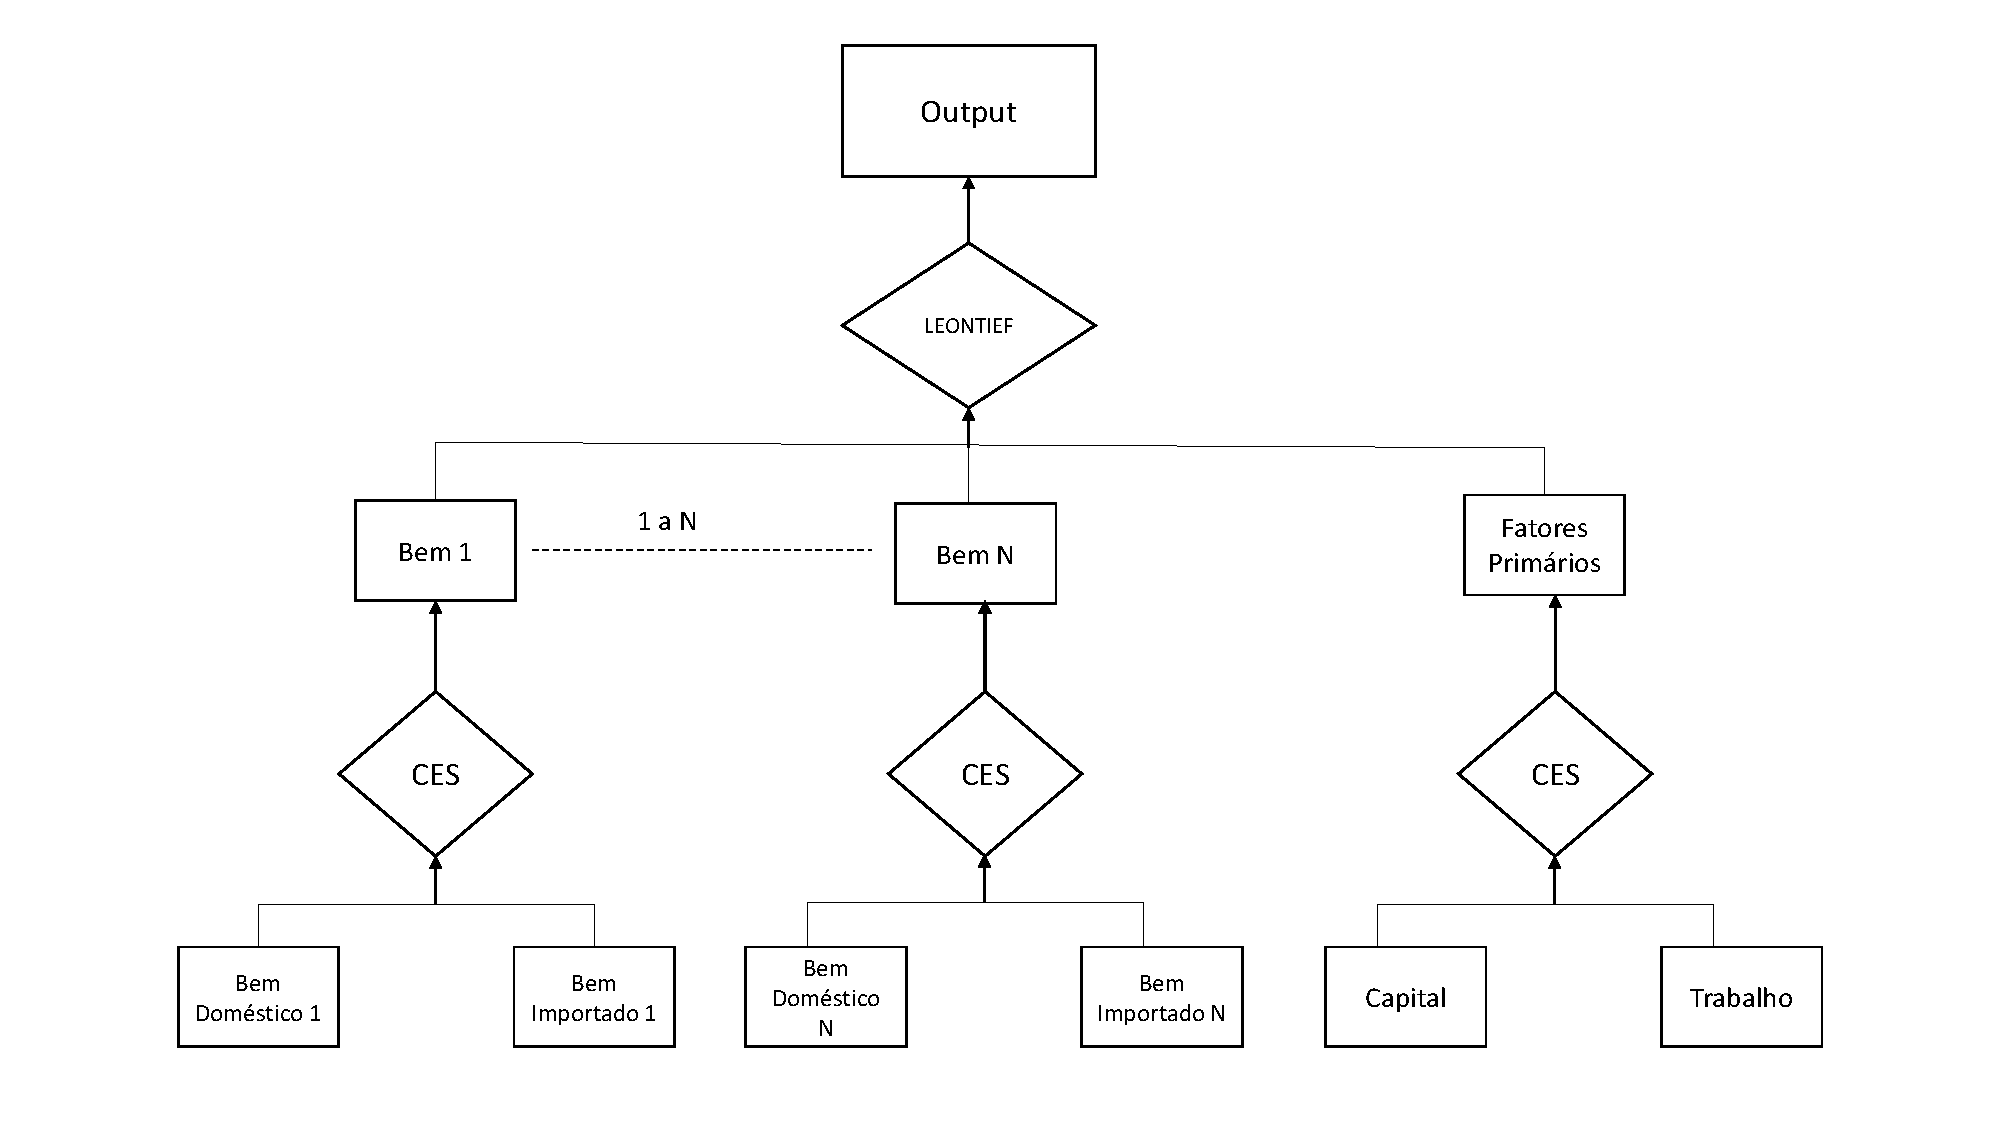
\includegraphics{producao.pdf}
\caption{Estrutura da Produção\label{producao1}}
\end{figure}

Para essa tecnologia, tem-se as seguintes funções de demanda:

\begin{itemize}
\item
  Demanda por bens intermediários (compostos)\footnote{Os bens
    intermediários compostos são uma composição entre produtos
    domésticos e importados.}:
  \[X^s_{ci} = A_{ci} \times \text{X1TOT}_i, ~i \in \text{IND},~c \in \text{COM}\]
\item
  Demanda por valor adicionado:
  \[\text{X1PRIM}_i = A\text{1PRIM}_{i}\times \text{X1TOT}_i\]
\end{itemize}

Essas equações, facilmente, podem ser reescritas em variações exatas:

\begin{itemize}
\item
  Demanda por bens intermediários:
  \[\hat{X}^s_{ci} = \hat{A}_{ci}\times \hat{\text{X1TOT}}_i, ~i \in \text{IND},~c \in \text{COM}\]
\item
  Demanda por valor adicionado:
  \[\hat{\text{X1PRIM}}_i = \hat{\text{A1PRIM}}_i \times \hat{\text{X1TOT}}_i\]
\end{itemize}

Na sequência, vamos definir os parâmetros \(\hat{A}_{ci}\) e
\(\hat{\text{A1PRIM}}_i\). Como estamos usando em variação, o valor
inicial desses parâmetros é igual a 1.

\begin{Shaded}
\begin{Highlighting}[]
\NormalTok{params[[}\StringTok{"A"}\NormalTok{]] <-}\StringTok{ }\KeywordTok{create_param}\NormalTok{(}
  \DataTypeTok{value =} \DecValTok{1}\NormalTok{,}
  \DataTypeTok{indexes =}\NormalTok{ sets[}\KeywordTok{c}\NormalTok{(}\StringTok{'COM'}\NormalTok{, }\StringTok{'IND'}\NormalTok{)],}
  \DataTypeTok{desc =} \StringTok{"Variação do coeficiente técnico para o produto c usado pela indústria i"}
\NormalTok{)}

\NormalTok{params[[}\StringTok{"A1PRIM"}\NormalTok{]] <-}\StringTok{ }\KeywordTok{create_param}\NormalTok{(}
  \DataTypeTok{value =} \DecValTok{1}\NormalTok{,}
  \DataTypeTok{indexes =}\NormalTok{ sets[}\StringTok{'IND'}\NormalTok{],}
  \DataTypeTok{desc =} \StringTok{"Variação do coeficiente técnico para o fator primário usado pela indústria i"}
\NormalTok{)}
\end{Highlighting}
\end{Shaded}

Agora, vamos definir as variáveis \(\hat{X}_{ci}\) (uso do produto
composto \(c\) pela indústria \(i\)) e \(\hat{\text{X1PRIM}}_i\) (uso do
fator primário composto). Aqui, existe um detalhe, o uso do produto
\(c\) pode ser feito pelas indústrias ou pelos demais usuários que
demandam importações (IMPUSER). Dessa forma, na definição da variável
\(\hat{X}_{ci}\), vamos utilizar o conjunto IMPUSER ao invés do conjunto
IND. Deixando mais claro, iremos definir

\[ \hat{X}^s_{cu},~ c \in \text{COM}, u \in \text{IMPUSER} \]
\[ \hat{X}^s_{cu} =
\begin{cases}
\hat{X}^s_{ci}       & \quad \text{se } u \in \text{IND}\\
\hat{X}^s_{c,\text{HH}}       & \quad \text{se } u = \text{Households}\\
\hat{X}^s_{c,\text{GOV}}       & \quad \text{se } u = \text{Governement}\\
\hat{X}^s_{c,\text{INV}}       & \quad \text{se } u = \text{Investment}
\end{cases}
\]

Ambas as variáveis são do tipo \emph{defined}, pois possuem equações que
definem os seus valores.

\begin{Shaded}
\begin{Highlighting}[]
\CommentTok{# chamamos de x de x_s (composto de várias sources s)}
\NormalTok{variables[[}\StringTok{"x_s"}\NormalTok{]] <-}\StringTok{ }\KeywordTok{create_variable}\NormalTok{(}
  \DataTypeTok{value =} \DecValTok{1}\NormalTok{,}
  \DataTypeTok{indexes =}\NormalTok{ sets[}\KeywordTok{c}\NormalTok{(}\StringTok{"COM"}\NormalTok{, }\StringTok{"IMPUSER"}\NormalTok{)],}
  \DataTypeTok{type =} \StringTok{"defined"}\NormalTok{,}
  \DataTypeTok{desc =} \StringTok{"Variação no uso do composto c por impuser"}
\NormalTok{)}

\NormalTok{variables[[}\StringTok{"x1prim"}\NormalTok{]] <-}\StringTok{ }\KeywordTok{create_variable}\NormalTok{(}
  \DataTypeTok{value =} \DecValTok{1}\NormalTok{,}
  \DataTypeTok{indexes =}\NormalTok{ sets[}\KeywordTok{c}\NormalTok{(}\StringTok{'IND'}\NormalTok{)],}
  \DataTypeTok{type =} \StringTok{"defined"}\NormalTok{,}
  \DataTypeTok{desc =} \StringTok{"Uso do fator primário composto por indústria"}
\StringTok{)}
\end{Highlighting}
\end{Shaded}

Finalmente, iremos definir as equações. Note que temos a equação de uso
para o produto composto c para os usuários industriais. Assim, iremos
utilizar o índice \texttt{i\ in\ IND} (\(i \in \text{IND}\)).

\begin{Shaded}
\begin{Highlighting}[]
\NormalTok{equations[[}\StringTok{"E_x_s_ind"}\NormalTok{]] <-}\StringTok{ }\KeywordTok{create_equation}\NormalTok{(}
  \StringTok{'x_s[c,i] = A[c,i] * x1tot[i]'}\NormalTok{,}
  \DataTypeTok{indexes =} \KeywordTok{c}\NormalTok{(}\StringTok{'c in COM'}\NormalTok{, }\StringTok{'i in IND'}\NormalTok{),}
  \DataTypeTok{type =} \StringTok{"defining"}\NormalTok{,}
  \DataTypeTok{desc =} \StringTok{"Variação do uso do composto c por indústria"}
\StringTok{)}
\end{Highlighting}
\end{Shaded}

\begin{Shaded}
\begin{Highlighting}[]
\NormalTok{equations[[}\StringTok{"E_x1prim"}\NormalTok{]] <-}\StringTok{ }\KeywordTok{create_equation}\NormalTok{(}
  \StringTok{'x1prim[i] = A1PRIM[i] * x1tot[i]'}\NormalTok{,}
  \DataTypeTok{indexes =} \StringTok{'i in IND'}\NormalTok{,}
  \DataTypeTok{type =} \StringTok{"defining"}\NormalTok{,}
  \DataTypeTok{desc =} \StringTok{"Uso do fator primário composto por indústria"}
\StringTok{)}
\end{Highlighting}
\end{Shaded}

Perceba que ainda não especificamos a variável \(\hat{\text{X1TOT}}_i\).
Ela será especificada em momento oportuno, mas vale antecipar que essa
variável é do tipo \texttt{mcc}. Por quê? Perceba que, na Equação
\ref{e_x1tot}, \(\text{X1TOT}_i\) é função dos usos de bens
intermediários e fatores primários. No entanto, a quantidade demandada
desses bens e fatores dependem de \(\text{X1TOT}\). Dessa forma,
\(\text{X1TOT}\) não pode ser definida. Precisaremos de uma condição de
equilibrio de mercado para encontrar o seu valor no novo equilíbrio.
Isto será feito posteriormente.

Adicionalmente, por enquanto, não entraremos nos detalhes sobre a
demanda no segundo nível (escolha entre bens domésticos e importados),
tendo em vista que a forma da demanda é comum independente do usuário
(indústrias, família, governo etc.).

\hypertarget{famuxedlias}{%
\subsubsection{Famílias}\label{famuxedlias}}

Para as famílias, que serão representadas como \emph{HH}, assume-se um
agente representativo com preferências do tipo Cobb-Douglas sobre um
conjunto de produtos (compostos) e uma restrição orçamentária. Isto é:
\[U = \prod_{c \in \text{COM}}{X^s_{c,\text{HH}}}^{\alpha_c}\]
\[s.a. \sum_{c\in \text{COM}} P_{c,\text{HH}} X^s_{c,\text{HH}} = \text{W3TOT},\]
em que \(X_{c,\text{HH}}\) é quantidade demandada do bem composto \(c\)
pelas famílias (\emph{HH}), \(P_{c,\text{HH}}\) é o índice de preço do
bem composto \(c\) para as famílias e \(\text{W3TOT}\) é renda nominal
das famílias. Adicionalmente, \(\sum_{c \in \text{COM}} \alpha_c = 1\).

Para esse tipo de preferência, sabe-se que, a partir da maximização de
utilidade do consumidor, a função de demanda ótima é:
\[X^s_{c,\text{HH}} = \alpha_c \frac{\text{W3TOT}}{P_{c,\text{HH}}},~ c \in \text{COM}.\]

Em variações, a demanda das famílias é escrita da seguinte forma:
\[\hat{X}^s_{c,\text{HH}} =  \frac{\hat{\text{W3TOT}}}{\hat{P}_{c,\text{HH}}}, ~ c \in \text{COM}.\]

Por fim, definimos o dispêndio real das famílias (\(\text{X3TOT}\))
como:
\[\hat{\text{X3TOT}} = \frac{\hat{\text{W3TOT}}}{\hat{\text{P3TOT}}},\]
em que \(\text{P3TOT}\) é o índice de preços associado à cesta de
consumo das famílias. Para uma função do tipo cobb-douglas, o índice
\(\text{P3TOT}\) pode ser definido como:

\[ \text{P3TOT} = \prod_{c \in COM} \left(\frac{P^s_{c,HH}}{\alpha_c}\right)^{\alpha_c}.\]

Em variação, esse índice é reescrito como:

\[ \hat{\text{P3TOT}} = \prod_{c \in COM} \left(\hat{P}^s_{c,HH}\right)^{\alpha_c},\]
em que \(\alpha_c\) é a participação do bem \(c\) no dispêndio das
famílias.

Especificado a estrutura das famílias no modelo, vamos definir,
primeiramente, o parâmetro \(\text{SHARE}_{c,\text{HH}}\).

\begin{Shaded}
\begin{Highlighting}[]
\CommentTok{# calcula os shares}
\NormalTok{SHARE_HH <-}\StringTok{ }\NormalTok{use_df }\OperatorTok\StringTok{ }
\StringTok{  }\KeywordTok{filter}\NormalTok{(USER }\OperatorTok{==}\StringTok{ "Households"}\NormalTok{) }\OperatorTok\StringTok{ }
\StringTok{  }\KeywordTok{group_by}\NormalTok{(COM) }\OperatorTok\StringTok{ }
\StringTok{  }\KeywordTok{summarise}\NormalTok{(}\DataTypeTok{Value =} \KeywordTok{sum}\NormalTok{(Value)) }\OperatorTok\StringTok{ }
\StringTok{  }\KeywordTok{mutate}\NormalTok{(}\DataTypeTok{SHARE =}\NormalTok{ Value}\OperatorTok{/}\KeywordTok{sum}\NormalTok{(Value)) }\OperatorTok\StringTok{ }
\StringTok{  }\KeywordTok{select}\NormalTok{(COM, SHARE)}

\NormalTok{params[[}\StringTok{"SHARE_HH"}\NormalTok{]] <-}\StringTok{ }\KeywordTok{create_param}\NormalTok{(}
  \DataTypeTok{value =}\NormalTok{ SHARE_HH,}
  \DataTypeTok{indexes =}\NormalTok{ sets[}\StringTok{'COM'}\NormalTok{],}
  \DataTypeTok{desc =} \StringTok{"Participação do bem c no dispêndio das famílias"}
\NormalTok{)}
\end{Highlighting}
\end{Shaded}

No fechamento do modelo que será adotado, o dispêndio real das famílias
(\(\hat{\text{X3TOT}}\)) será exógeno. Portanto, o definiremos como um
parâmetro do modelo.

\begin{Shaded}
\begin{Highlighting}[]
\NormalTok{params[[}\StringTok{"X3TOT"}\NormalTok{]] <-}\StringTok{ }\KeywordTok{create_param}\NormalTok{(}
  \DataTypeTok{value =} \DecValTok{1}\NormalTok{,}
  \DataTypeTok{indexes =} \StringTok{"X3TOT"}\NormalTok{,}
  \DataTypeTok{desc =} \StringTok{"Variação no dispêndio real das famílias"}
\NormalTok{)}
\end{Highlighting}
\end{Shaded}

Com essa definição, temos que:
\[\hat{\text{W3TOT}} = \hat{\text{X3TOT}} \times \hat{\text{P3TOT}}.\]
Isto é, a variação da renda das famílias tem que ser igual a variação do
dispêndio real vezes a variação dos preços para as famílias.

Lembrando que a variável \(\hat{X}_{c,\text{HH}}\) já está incluída na
variável \texttt{x\_s}, vamos definir as demais variáveis desse bloco:

\begin{Shaded}
\begin{Highlighting}[]
\NormalTok{variables[[}\StringTok{"p3tot"}\NormalTok{]] <-}\StringTok{ }\KeywordTok{create_variable}\NormalTok{(}
  \DataTypeTok{value =} \DecValTok{1}\NormalTok{,}
  \DataTypeTok{indexes =} \StringTok{"p3tot"}\NormalTok{,}
  \DataTypeTok{type =} \StringTok{"defined"}\NormalTok{,}
  \DataTypeTok{desc =} \StringTok{"Variação no índice de preços das famílias"}
\NormalTok{)}

\NormalTok{variables[[}\StringTok{"w3tot"}\NormalTok{]] <-}\StringTok{ }\KeywordTok{create_variable}\NormalTok{(}
  \DataTypeTok{value =} \DecValTok{1}\NormalTok{,}
  \DataTypeTok{indexes =} \StringTok{"w3tot"}\NormalTok{,}
  \DataTypeTok{type =} \StringTok{"defined"}\NormalTok{,}
  \DataTypeTok{desc =} \StringTok{"Variação da renda nominal das famílias"}
\NormalTok{)}
\end{Highlighting}
\end{Shaded}

Finalmente, vamos definir as equações:

\begin{Shaded}
\begin{Highlighting}[]
\NormalTok{equations[[}\StringTok{"E_p3tot"}\NormalTok{]] <-}\StringTok{ }\KeywordTok{create_equation}\NormalTok{(}
  \StringTok{'p3tot = prod(p_s[,"Households"]^SHARE_HH[])'}\NormalTok{,}
  \DataTypeTok{type =} \StringTok{"defining"}\NormalTok{,}
  \DataTypeTok{desc =} \StringTok{"Variação do índice de preços das famílias"}
\NormalTok{)}

\NormalTok{equations[[}\StringTok{"E_w3tot"}\NormalTok{]] <-}\StringTok{ }\KeywordTok{create_equation}\NormalTok{(}
  \StringTok{'w3tot = X3TOT * p3tot'}\NormalTok{,}
  \DataTypeTok{type =} \StringTok{"defining"}\NormalTok{,}
  \DataTypeTok{desc =} \StringTok{"Variação na renda (dispêndio) nominal das família"}
\NormalTok{)}

\NormalTok{equations[[}\StringTok{"E_x_s_hh"}\NormalTok{]] <-}\StringTok{ }\KeywordTok{create_equation}\NormalTok{(}
  \StringTok{'x_s[c, "Households"] = w3tot/p_s[c, "Households"]'}\NormalTok{,}
  \DataTypeTok{indexes =} \KeywordTok{c}\NormalTok{(}\StringTok{'c in COM'}\NormalTok{),}
  \DataTypeTok{type =} \StringTok{"defining"}\NormalTok{,}
  \DataTypeTok{desc =} \StringTok{"Variação do uso do composto c pelas famílias"}
\NormalTok{)}
\end{Highlighting}
\end{Shaded}

\hypertarget{investimento-e-governo}{%
\subsubsection{Investimento e Governo}\label{investimento-e-governo}}

No MINIMAL, não é assumida nenhuma estrutura específica para o dispêndio
em investimento ou do governo. Será assumido, que essas duas fontes de
demandas são exógenas. Ou seja, \(\hat{X}^s_{c,\text{INV}} = 1\) e
\(\hat{X}^s_{c,\text{GOV}} = 1\). Portanto, iremos apenas defini-los
como parâmetros, que poderão ser utilizados posteriormente como fontes
de choques do modelo.

\begin{Shaded}
\begin{Highlighting}[]
\NormalTok{params[[}\StringTok{"X_S_INV"}\NormalTok{]] <-}\StringTok{ }\KeywordTok{create_param}\NormalTok{(}
  \DataTypeTok{value =} \DecValTok{1}\NormalTok{,}
  \DataTypeTok{indexes =}\NormalTok{ sets[}\StringTok{"COM"}\NormalTok{],}
  \DataTypeTok{desc =} \StringTok{"Variação na demanda de investimento por produto c"}
\NormalTok{)}

\NormalTok{params[[}\StringTok{"X_S_GOV"}\NormalTok{]] <-}\StringTok{ }\KeywordTok{create_param}\NormalTok{(}
  \DataTypeTok{value =} \DecValTok{1}\NormalTok{,}
  \DataTypeTok{indexes =}\NormalTok{ sets[}\StringTok{"COM"}\NormalTok{],}
  \DataTypeTok{desc =} \StringTok{"Variação na demanda do governo por produto c"}
\NormalTok{)}
\end{Highlighting}
\end{Shaded}

Também definimos as equações que capturarão esses choques.

\begin{Shaded}
\begin{Highlighting}[]
\NormalTok{equations[[}\StringTok{"E_x_s_inv"}\NormalTok{]] <-}\StringTok{ }\KeywordTok{create_equation}\NormalTok{(}
  \StringTok{'x_s[c, "Investment"] = X_S_INV[c]'}\NormalTok{,}
  \DataTypeTok{indexes =} \StringTok{'c in COM'}\NormalTok{,}
  \DataTypeTok{type =} \StringTok{"defining"}\NormalTok{,}
  \DataTypeTok{desc =} \StringTok{"Variação no uso do composto c para investimento"}
\NormalTok{)}

\NormalTok{equations[[}\StringTok{"E_x_s_gov"}\NormalTok{]] <-}\StringTok{ }\KeywordTok{create_equation}\NormalTok{(}
  \StringTok{'x_s[c, "Government"] = X_S_GOV[c]'}\NormalTok{,}
  \DataTypeTok{indexes =} \StringTok{'c in COM'}\NormalTok{,}
  \DataTypeTok{type =} \StringTok{"defining"}\NormalTok{,}
  \DataTypeTok{desc =} \StringTok{"Variação no uso do composto c pelo governo"}
\NormalTok{)}
\end{Highlighting}
\end{Shaded}

\hypertarget{demanda-de-segundo-nuxedvel-entre-bens-domuxe9sticos-e-importados}{%
\subsubsection{Demanda de segundo nível entre bens domésticos e
importados}\label{demanda-de-segundo-nuxedvel-entre-bens-domuxe9sticos-e-importados}}

Até o momento, apresentamos a demanda\footnote{O componente de
  exportação demanda apenas o bem doméstico.} das indústrias, das
famílias, do governo e do investimento pelos bens compostos. Nessa
parte, vamos definir a demanda do nível inferior. Nesse nível, o
consumidor escolhe alocar o seu consumo total entre o produto doméstico
e o produto importado.

É assumida uma função de agregação CES, com elasticidade de substituição
\(\sigma_i\), que combina os produtos domésticos e importados. Nesse
caso, a variação na demanda por cada produto, por fonte e por usuário,
\(\hat{X}_{csu}\), é dada pela seguinte função de demanda:
\begin{equation}\label{e_x}
\hat{X}_{csu} = \left(\frac{\hat{P}_{cs}}{\hat{P}^s_{cu}}\right)^{-\sigma_c} \hat{X}^s_{cu}, \quad c \in \text{COM},~s \in \text{SRC},~s \in \text{IMPUSER}
\end{equation} em que \(\hat{P}_{cs}\) é a variação do preço do produto
\(c\) fornecido pela fonte \(s\). Já \(\hat{P}^s_{cu}\) é o índice de
preço do bem composto \(c\) para o usuário \(u\).

Abaixo, define-se a variável \(\hat{X}_{csu}\) e a equação para os
usuários pertencentes ao conjunto IMPUSER.

\begin{Shaded}
\begin{Highlighting}[]
\NormalTok{variables[[}\StringTok{"x"}\NormalTok{]] <-}\StringTok{ }\KeywordTok{create_variable}\NormalTok{(}
  \DataTypeTok{value =} \DecValTok{1}\NormalTok{,}
  \DataTypeTok{indexes =}\NormalTok{ sets[}\KeywordTok{c}\NormalTok{(}\StringTok{"COM"}\NormalTok{,}\StringTok{"SRC"}\NormalTok{,}\StringTok{"USER"}\NormalTok{)],}
  \DataTypeTok{type =} \StringTok{"defined"}\NormalTok{,}
  \DataTypeTok{desc =} \StringTok{"Variação na demanda por produto, fonte e usuário"}
\NormalTok{)}

\NormalTok{equations[[}\StringTok{"E_x_impuser"}\NormalTok{]] <-}\StringTok{ }\KeywordTok{create_equation}\NormalTok{(}
  \StringTok{'x[c,s,u] = x_s[c,u]*(p[c,s]/p_s[c,u])^(-SIGMA[c])'}\NormalTok{,}
  \DataTypeTok{indexes =} \KeywordTok{c}\NormalTok{(}\StringTok{'c in COM'}\NormalTok{, }\StringTok{'s in SRC'}\NormalTok{, }\StringTok{'u in IMPUSER'}\NormalTok{),}
  \DataTypeTok{type =} \StringTok{"defining"}\NormalTok{,}
  \DataTypeTok{desc =} \StringTok{"Variação na demanda por produto, fonte e usuário"}
\NormalTok{)}
\end{Highlighting}
\end{Shaded}

Perceba que a variável foi definida para todos os usuários. No entanto,
na Equação \ref{e_x}, está definida equação para
\(u \in \text{IMPUSER}\). Isto deve-se ao fato de que a demanda para o
usuário \emph{Exports} será definida de outra forma.

\hypertarget{exportauxe7uxf5es}{%
\subsubsection{Exportações}\label{exportauxe7uxf5es}}

Para as exportações, é assumida uma função de elasticidade constante com
parâmetro \(\text{EXP\_ELAST}_c\) para o produto \(c\). A demanda
externa pelo produto doméstico depende do preço relativo entre o preço
doméstico e o preço internacional daquele produto:
\[\hat{X}_{csu} = \hat{F4Q}_c \left(\frac{\hat{P}_{cs}}{\hat{\phi}~\hat{\text{PWORLD}_c}}\right)^{-\text{EXP ELAST}_c}, \quad c \in \text{COM},~s = \text{dom},~u=\text{Exports}\]
em que \(\hat{F4Q}_c\) é um \emph{shift} na demanda externa.

Abaixo, definimos este bloco.

\begin{Shaded}
\begin{Highlighting}[]
\NormalTok{params[[}\StringTok{"EXP_ELAST"}\NormalTok{]] <-}\StringTok{ }\KeywordTok{create_param}\NormalTok{(}
  \DataTypeTok{value =}\NormalTok{ p018_df,}
  \DataTypeTok{indexes =}\NormalTok{ sets[}\StringTok{"COM"}\NormalTok{],}
  \DataTypeTok{desc =} \StringTok{"Elasticidade da demanda por exportações"}
\NormalTok{)}

\NormalTok{params[[}\StringTok{"F4Q"}\NormalTok{]] <-}\StringTok{ }\KeywordTok{create_param}\NormalTok{(}
  \DataTypeTok{value =} \DecValTok{1}\NormalTok{,}
  \DataTypeTok{indexes =}\NormalTok{ sets[}\KeywordTok{c}\NormalTok{(}\StringTok{"COM"}\NormalTok{)],}
  \DataTypeTok{desc =} \StringTok{"Shift na demanda externa para o produto c"}
\NormalTok{)}

\NormalTok{equations[[}\StringTok{"E_x_exp"}\NormalTok{]] <-}\StringTok{ }\KeywordTok{create_equation}\NormalTok{(}
  \StringTok{'x[c,"dom","Exports"] = F4Q[c]*(p[c,"dom"]/(PHI*PWORLD[c]))^(-EXP_ELAST[c])'}\NormalTok{,}
  \DataTypeTok{indexes =} \StringTok{'c in COM'}\NormalTok{,}
  \DataTypeTok{type =} \StringTok{"defining"}\NormalTok{,}
  \DataTypeTok{desc =} \StringTok{"Variação das exportações do produto c"}
\NormalTok{)}
\end{Highlighting}
\end{Shaded}

\hypertarget{demanda-por-fatores-primuxe1rios}{%
\subsubsection{Demanda por Fatores
Primários}\label{demanda-por-fatores-primuxe1rios}}

Na parte da produção, vimos como cada indústria define a quantidade de
fator primário que será utilizada para atingir uma determinada produção.
Todavia, cada indústria pode escolher um mix diferente entre os fatores
de produção capital e trabalho. Para essa alocação, também é utilizada
uma função de agregação CES, com elasticidade substituição
\(\sigma^{1PRIM}_i\). Assim, pode-se definir a demanda (em variações)
por trabalho e capital na indústria \(i\) como:
\[\hat{\text{X1LAB}}_i = \left(\frac{\hat{\text{P1LAB}}}{\hat{\text{P1PRIM}}_i}\right)^{-\sigma_i^{\text{1PRIM}}}\hat{\text{X1PRIM}}_i, \quad i \in \text{IND} \quad \text{e}\]
\[\hat{\text{X1CAP}}_i = \left(\frac{\hat{\text{P1CAP}}_i}{\hat{\text{P1PRIM}}_i}\right)^{-\sigma_i^{\text{1PRIM}}}\hat{\text{X1PRIM}}_i, \quad i \in \text{IND},\]
em que \(\hat{\text{X1LAB}}_i\) é a variação da demanda por trabalho
pela indústria \(i\), \(\hat{\text{P1LAB}}\) é o salário nominal,
\(\hat{\text{P1PRIM}}_i\) é a variação do índice de preços dos fatores
primários para a indústria \(i\), \(\hat{\text{X1PRIM}}_i\) é a variação
da demanda por fatores primários da indústria \(i\),
\(\hat{\text{X1CAP}}_i\) é a variação da demanda por capital pela
indústria \(i\) e \(\hat{\text{P1CAP}}_i\) é a remuneração do capital na
indústria \(i\).

Considerando que os fatores primários são agregados a partir de uma
função do tipo CES, a variável \(\hat{\text{P1PRIM}}_i\) é calculada da
seguinte forma:
\[\hat{\text{P1PRIM}}_i = \left[\text{SHAREPRIM}_{\text{lab},i}\times \hat{\text{P1LAB}}^{1 - \sigma_i^{\text{1prim}}} + \text{SHAREPRIM}_{\text{cap},i}\times \hat{\text{P1CAP}}^{1 - \sigma_i^{\text{1prim}}}_i\right]^\frac{1}{1 - \sigma_i^{\text{1prim}}}\]

Note que o índice da \(i\) foi retirado de \(\hat{\text{P1LAB}}\)
(salário), pois no fechamento adotado assume-se que o trabalho tem
perfeita mobilidade entre os setores. Diferentemente, o capital será
assumido fixo dentro de cada indústria. Ademais, consideraremos que no
curto prazo a variação do salário real (\(\hat{\text{RW}}\)) é fixa
(exógena) e a variação do nível de emprego (\(\hat{L}\)) é endógena, o
que implica que \(\hat{\text{P1LAB}}\) deve variar na mesma proporção de
\(\hat{\text{P3TOT}}\). Então, temos a seguinte equação:
\[\hat{\text{P1LAB}} = \hat{\text{RW}} \times \hat{\text{P3TOT}}\]
Primeiro, definimos os parâmetros desse bloco.

\begin{Shaded}
\begin{Highlighting}[]
\NormalTok{params[[}\StringTok{"SIGMA1PRIM"}\NormalTok{]] <-}\StringTok{ }\KeywordTok{create_param}\NormalTok{(}
  \DataTypeTok{value =}\NormalTok{ p028_df,}
  \DataTypeTok{indexes =}\NormalTok{ sets[}\StringTok{"IND"}\NormalTok{],}
  \DataTypeTok{desc =} \StringTok{"Elasticidade de subsituição entre os fatores de produção"}
\NormalTok{)}

\NormalTok{SHAREPRIM <-}\StringTok{ }\NormalTok{fac_df }\OperatorTok\StringTok{ }
\StringTok{  }\KeywordTok{group_by}\NormalTok{(IND) }\OperatorTok\StringTok{ }
\StringTok{  }\KeywordTok{mutate}\NormalTok{(}\DataTypeTok{SHAREPRIM =}\NormalTok{ Value}\OperatorTok{/}\KeywordTok{sum}\NormalTok{(Value)) }\OperatorTok\StringTok{ }
\StringTok{  }\KeywordTok{select}\NormalTok{(FAC, IND, SHAREPRIM)}

\NormalTok{params[[}\StringTok{"SHAREPRIM"}\NormalTok{]] <-}\StringTok{ }\KeywordTok{create_param}\NormalTok{(}
  \DataTypeTok{value =}\NormalTok{ SHAREPRIM,}
  \DataTypeTok{indexes =}\NormalTok{ sets[}\KeywordTok{c}\NormalTok{(}\StringTok{"FAC"}\NormalTok{, }\StringTok{"IND"}\NormalTok{)],}
  \DataTypeTok{desc =} \StringTok{"Part. de cada fator no uso do fator primário por indústria"}
\StringTok{)}
\end{Highlighting}
\end{Shaded}

\begin{Shaded}
\begin{Highlighting}[]
\NormalTok{params[[}\StringTok{"RW"}\NormalTok{]] <-}\StringTok{ }\KeywordTok{create_param}\NormalTok{(}
  \DataTypeTok{value =} \DecValTok{1}\NormalTok{,}
  \DataTypeTok{indexes =} \StringTok{"rw"}\NormalTok{,}
  \DataTypeTok{desc =} \StringTok{'Variação no salário real'}
\NormalTok{)}
\end{Highlighting}
\end{Shaded}

Na sequência, definimos as variáveis.

\begin{Shaded}
\begin{Highlighting}[]
\NormalTok{variables[[}\StringTok{"x1lab"}\NormalTok{]] <-}\StringTok{ }\KeywordTok{create_variable}\NormalTok{(}
  \DataTypeTok{value =} \DecValTok{1}\NormalTok{,}
  \DataTypeTok{indexes =}\NormalTok{ sets[}\KeywordTok{c}\NormalTok{(}\StringTok{'IND'}\NormalTok{)],}
  \DataTypeTok{type =} \StringTok{"defined"}\NormalTok{,}
  \DataTypeTok{desc =} \StringTok{"Variação no emprego por indústria"}
\StringTok{)}

\StringTok{variables[["}\NormalTok{x1cap}\StringTok{"]] <- create_variable(}
\StringTok{  value = 1,}
\StringTok{  indexes = sets[c('IND')],}
\StringTok{  type = "}\NormalTok{defined}\StringTok{",}
\StringTok{  desc = "}\NormalTok{Variação no uso de capital por indústria"}
\NormalTok{)}
\end{Highlighting}
\end{Shaded}

\begin{Shaded}
\begin{Highlighting}[]
\NormalTok{variables[[}\StringTok{"p1lab"}\NormalTok{]] <-}\StringTok{ }\KeywordTok{create_variable}\NormalTok{(}
  \DataTypeTok{value =} \DecValTok{1}\NormalTok{,}
  \DataTypeTok{indexes =} \StringTok{"p1lab"}\NormalTok{,}
  \DataTypeTok{type =} \StringTok{"defined"}\NormalTok{,}
  \DataTypeTok{desc =} \StringTok{"Variação no salário nominal"}
\NormalTok{)}


\NormalTok{variables[[}\StringTok{"p1prim"}\NormalTok{]] <-}\StringTok{ }\KeywordTok{create_variable}\NormalTok{(}
  \DataTypeTok{value =} \DecValTok{1}\NormalTok{,}
  \DataTypeTok{indexes =}\NormalTok{ sets[}\StringTok{'IND'}\NormalTok{],}
  \DataTypeTok{type =} \StringTok{"defined"}\NormalTok{,}
  \DataTypeTok{desc =} \StringTok{"Variação no índice de preço do fator primário composto por indústria i"}
\NormalTok{)}
\end{Highlighting}
\end{Shaded}

Por fim, vamos definir as equações.

\begin{Shaded}
\begin{Highlighting}[]
\NormalTok{equations[[}\StringTok{"E_x1lab"}\NormalTok{]] <-}\StringTok{ }\KeywordTok{create_equation}\NormalTok{(}
  \StringTok{'x1lab[i] = x1prim[i]*(p1lab/p1prim[i])^(-SIGMA1PRIM[i])'}\NormalTok{,}
  \DataTypeTok{indexes =} \KeywordTok{c}\NormalTok{(}\StringTok{'i in IND'}\NormalTok{),}
  \DataTypeTok{type =} \StringTok{"defining"}\NormalTok{,}
  \DataTypeTok{desc =} \StringTok{"Variação no emprego por indústria"}
\StringTok{)}
\end{Highlighting}
\end{Shaded}

\begin{Shaded}
\begin{Highlighting}[]
\NormalTok{equations[[}\StringTok{"E_p1lab"}\NormalTok{]] <-}\StringTok{ }\KeywordTok{create_equation}\NormalTok{(}
  \StringTok{'p1lab = RW * p3tot'}\NormalTok{,}
  \DataTypeTok{type =} \StringTok{"defining"}\NormalTok{,}
  \DataTypeTok{desc =} \StringTok{"Variação no salário nominal"}
\NormalTok{)}

\NormalTok{equations[[}\StringTok{"E_x1cap"}\NormalTok{]] <-}\StringTok{ }\KeywordTok{create_equation}\NormalTok{(}
  \StringTok{'x1cap[i] = (p1cap[i]/p1prim[i])^(-SIGMA1PRIM[i]) * x1prim[i]'}\NormalTok{,}
  \DataTypeTok{indexes =} \StringTok{"i in IND"}\NormalTok{,}
  \DataTypeTok{type =} \StringTok{"defining"}\NormalTok{,}
  \DataTypeTok{desc =} \StringTok{"Variação na demanda por capital na indústria i"}
\NormalTok{)}

\NormalTok{equations[[}\StringTok{"E_p1prim"}\NormalTok{]] <-}\StringTok{ }\KeywordTok{create_equation}\NormalTok{(}
  \StringTok{'p1prim[i] = (SHAREPRIM["Labour", i] * p1lab^(1 - SIGMA1PRIM[i]) +}
\StringTok{    SHAREPRIM["Capital", i] * p1cap[i]^(1 - SIGMA1PRIM[i]))^(1/(1-SIGMA1PRIM[i]))'}\NormalTok{,}
  \DataTypeTok{indexes =} \KeywordTok{c}\NormalTok{(}\StringTok{'i in IND'}\NormalTok{),}
  \DataTypeTok{type =} \StringTok{"defining"}\NormalTok{,}
  \DataTypeTok{desc =} \StringTok{"Variação no índice de preço do fator primário para indústria i"}
\NormalTok{)}
\end{Highlighting}
\end{Shaded}

\hypertarget{equiluxedbrios-nos-mercados-de-bens}{%
\subsubsection{Equilíbrios nos Mercados de
Bens}\label{equiluxedbrios-nos-mercados-de-bens}}

Para começar a especificar as condições de equilíbrio nos mercados de
bens, precisamos definir a demanda total por cada produto \(c\) para
cada fonte \(s\), \(\hat{X}^0_{cs}\):

\[\hat{X}^0_{cs} = \sum_{u \in \text{USER}} \text{SHRSALES}_{csu} \hat{X}_{csu}, \quad  c \in \text{COM}, s \in \text{SRC}\]
em que
\[\text{SHRSALES}_{csu} = \frac{\text{USE}_{csu}}{\sum_u\text{USE}_{csu}}, \quad  c \in \text{COM}, s \in \text{SRC}, u \in \text{USER}.\]
\(\text{USE}_{csu}\) é o valor da demanda de produto \(c\) da fonte
\(s\) pelo usuário \(u\).

Adicionalmente, pode-se definir a variação no custo de produção como:

\[\hat{\text{COST}}_i = \frac{\sum_c USE_{ci}^s \times \hat{P}^s_{ci} + \text{FAC}_{labour,i} \times \hat{\text{P1LAB}}_i + \text{FAC}_{capital,i} \times \hat{\text{P1CAP}_i}}{\text{V1TOT}_i},\]
em que \(USE_{ci}^s\) é o consumo total do produto \(c\) pela indústria
\(i\), \(\text{FAC}_{labour,i}\) é a remuneração total do fator trabalho
utilizado na indústria \(i\), \(\text{FAC}_{labour,i}\) é a remuneração
total do fator capital utilizado na indústria \(i\) e \text{V1TOT}\_i\$
é o custo total de produção da indústria \(i\) nos dados base.

O código abaixo cria os dados e define os parâmetros
\texttt{\textbackslash{}text\{SHRSALES\}\_\{csu\}}, \(\text{V1TOT}_i\),
\(\text{FAC}_{labour,i}\) e \(\text{FAC}_{capital,i}\).

\begin{Shaded}
\begin{Highlighting}[]
\NormalTok{SHRSALES <-}\StringTok{ }\NormalTok{use_df }\OperatorTok\StringTok{ }
\StringTok{  }\KeywordTok{group_by}\NormalTok{(COM, SRC) }\OperatorTok\StringTok{ }
\StringTok{  }\KeywordTok{mutate}\NormalTok{(}\DataTypeTok{SALES =} \KeywordTok{sum}\NormalTok{(Value),}
         \DataTypeTok{SHRSALES =}\NormalTok{ Value}\OperatorTok{/}\NormalTok{SALES) }\OperatorTok\StringTok{ }
\StringTok{  }\KeywordTok{select}\NormalTok{(COM, SRC, USER, SHRSALES)}

\NormalTok{use_s_df <-}\StringTok{ }\NormalTok{use_df }\OperatorTok\StringTok{ }
\StringTok{  }\KeywordTok{group_by}\NormalTok{(COM, USER) }\OperatorTok\StringTok{ }
\StringTok{  }\KeywordTok{summarise}\NormalTok{(}\DataTypeTok{Value =} \KeywordTok{sum}\NormalTok{(Value))}


\CommentTok{# Salários + Remuneração do Capital}
\NormalTok{V1PRIM <-}\StringTok{ }\NormalTok{fac_df }\OperatorTok\StringTok{ }
\StringTok{  }\KeywordTok{group_by}\NormalTok{(IND) }\OperatorTok\StringTok{ }
\StringTok{  }\KeywordTok{summarise}\NormalTok{(}\DataTypeTok{Value =} \KeywordTok{sum}\NormalTok{(Value))}

\CommentTok{# Custos Intermediários}
\NormalTok{IC <-}\StringTok{ }\NormalTok{use_df }\OperatorTok\StringTok{ }
\StringTok{  }\KeywordTok{filter}\NormalTok{(USER }\OperatorTok\StringTok{ }\NormalTok{IND) }\OperatorTok\StringTok{ }
\StringTok{  }\KeywordTok{group_by}\NormalTok{(}\DataTypeTok{IND =}\NormalTok{ USER) }\OperatorTok\StringTok{ }
\StringTok{  }\KeywordTok{summarise}\NormalTok{(}\DataTypeTok{ic =} \KeywordTok{sum}\NormalTok{(Value)) }

\CommentTok{# Custos totais}
\NormalTok{V1TOT <-}\StringTok{ }\NormalTok{V1PRIM }\OperatorTok\StringTok{ }
\StringTok{  }\KeywordTok{rename}\NormalTok{(}\DataTypeTok{va =}\NormalTok{ Value) }\OperatorTok\StringTok{ }
\StringTok{  }\KeywordTok{left_join}\NormalTok{(IC, }\DataTypeTok{by =} \StringTok{"IND"}\NormalTok{) }\OperatorTok\StringTok{ }
\StringTok{  }\KeywordTok{mutate}\NormalTok{(}\DataTypeTok{Value =}\NormalTok{ va }\OperatorTok{+}\StringTok{ }\NormalTok{ic) }\OperatorTok\StringTok{ }
\StringTok{  }\KeywordTok{select}\NormalTok{(IND, Value)}


\NormalTok{params[[}\StringTok{"USE"}\NormalTok{]] <-}\StringTok{ }\KeywordTok{create_param}\NormalTok{(}
  \DataTypeTok{value =}\NormalTok{ use_df,}
  \DataTypeTok{indexes =}\NormalTok{ sets[}\KeywordTok{c}\NormalTok{(}\StringTok{"COM"}\NormalTok{, }\StringTok{"SRC"}\NormalTok{, }\StringTok{"USER"}\NormalTok{)],}
  \DataTypeTok{desc =} \StringTok{"Uso do produto c da fonte s pelo usuário u"}
\NormalTok{)}

\NormalTok{params[[}\StringTok{"USE_S"}\NormalTok{]] <-}\StringTok{ }\KeywordTok{create_param}\NormalTok{(}
  \DataTypeTok{value =}\NormalTok{ use_s_df,}
  \DataTypeTok{indexes =}\NormalTok{ sets[}\KeywordTok{c}\NormalTok{(}\StringTok{"COM"}\NormalTok{, }\StringTok{"USER"}\NormalTok{)],}
  \DataTypeTok{desc =} \StringTok{"Uso do produto c da fonte s pelo usuário u"}
\NormalTok{)}

\NormalTok{params[[}\StringTok{"FAC0"}\NormalTok{]] <-}\StringTok{ }\KeywordTok{create_param}\NormalTok{(}
  \DataTypeTok{value =}\NormalTok{ fac_df,}
  \DataTypeTok{indexes =}\NormalTok{ sets[}\KeywordTok{c}\NormalTok{(}\StringTok{"FAC"}\NormalTok{, }\StringTok{"IND"}\NormalTok{)],}
  \DataTypeTok{desc =} \StringTok{"Uso inicial dos fatores primários pela indústria i"}
\NormalTok{)}

\NormalTok{params[[}\StringTok{"V1TOT"}\NormalTok{]] <-}\StringTok{ }\KeywordTok{create_param}\NormalTok{(}
  \DataTypeTok{value =}\NormalTok{ V1TOT,}
  \DataTypeTok{indexes =}\NormalTok{ sets[}\KeywordTok{c}\NormalTok{(}\StringTok{"IND"}\NormalTok{)],}
  \DataTypeTok{desc =} \StringTok{"Custo total da indústria i"}
\NormalTok{)}

\NormalTok{params[[}\StringTok{"SHRSALES"}\NormalTok{]] <-}\StringTok{ }\KeywordTok{create_param}\NormalTok{(}
  \DataTypeTok{value =}\NormalTok{ SHRSALES,}
  \DataTypeTok{indexes =}\NormalTok{ sets[}\KeywordTok{c}\NormalTok{(}\StringTok{"COM"}\NormalTok{, }\StringTok{"SRC"}\NormalTok{, }\StringTok{"USER"}\NormalTok{)],}
  \DataTypeTok{desc =} \StringTok{"Participação do usuário u nas vendas de c de origem s"}
\NormalTok{)}
\end{Highlighting}
\end{Shaded}

Com os parâmetros definidos, iremos adicionar as variáveis e as
equações.

\begin{Shaded}
\begin{Highlighting}[]
\NormalTok{variables[[}\StringTok{"x0"}\NormalTok{]] <-}\StringTok{ }\KeywordTok{create_variable}\NormalTok{(}
  \DataTypeTok{value =} \DecValTok{1}\NormalTok{,}
  \DataTypeTok{indexes =}\NormalTok{ sets[}\KeywordTok{c}\NormalTok{(}\StringTok{"COM"}\NormalTok{, }\StringTok{"SRC"}\NormalTok{)],}
  \DataTypeTok{type =} \StringTok{"defined"}\NormalTok{,}
  \DataTypeTok{desc =} \StringTok{"Variação na demanda total de c de origem s"}
\NormalTok{)}

\NormalTok{variables[[}\StringTok{"cost"}\NormalTok{]] <-}\StringTok{ }\KeywordTok{create_variable}\NormalTok{(}
  \DataTypeTok{value =} \DecValTok{1}\NormalTok{,}
  \DataTypeTok{indexes =}\NormalTok{ sets[}\KeywordTok{c}\NormalTok{(}\StringTok{"IND"}\NormalTok{)],}
  \DataTypeTok{type =} \StringTok{"defined"}\NormalTok{,}
  \DataTypeTok{desc =} \StringTok{"Variação no custo marginal de produção "}
\NormalTok{)}
\end{Highlighting}
\end{Shaded}

\begin{Shaded}
\begin{Highlighting}[]
\NormalTok{equations[[}\StringTok{"E_x0"}\NormalTok{]] <-}\StringTok{ }\KeywordTok{create_equation}\NormalTok{(}
  \StringTok{"x0[c,s] = sum(SHRSALES[c,s,] * x[c,s,])"}\NormalTok{,}
  \DataTypeTok{indexes =} \KeywordTok{c}\NormalTok{(}\StringTok{"c in COM"}\NormalTok{, }\StringTok{"s in SRC"}\NormalTok{),}
  \DataTypeTok{type =} \StringTok{"defining"}\NormalTok{,}
  \DataTypeTok{desc =} \StringTok{"Variação na demanda total de c de origem s"}
\NormalTok{)}

\NormalTok{equations[[}\StringTok{"E_cost"}\NormalTok{]] <-}\StringTok{ }\KeywordTok{create_equation}\NormalTok{(}
  \StringTok{"cost[i] = (sum(USE_S[,i] * p_s[,i]) +}
\StringTok{                  sum(FAC0[,i]) *p1prim[i])/(V1TOT[i])"}\NormalTok{,}
  \DataTypeTok{indexes =} \KeywordTok{c}\NormalTok{(}\StringTok{"i in IND"}\NormalTok{),}
  \DataTypeTok{type =} \StringTok{"defining"}\NormalTok{,}
  \DataTypeTok{desc =} \StringTok{"Variação no custo marginal de produção da indústria i"}
\NormalTok{)}
\end{Highlighting}
\end{Shaded}

Agora, vamos definir as equações para duas variáveis do tipo mcc:
\(\hat{\text{P1TOT}}_i\) e \(\hat{\text{X1TOT}}_i\):

\begin{itemize}
\item
  Condição de lucro zero para a indústria \(i\):
  \[\hat{\text{P1TOT}}_i = \hat{\text{COST}}_i, \quad i \in \text{IND}\]
\item
  Oferta igual a demanda para a indústria \(i\)\footnote{Lembre que o
    conjunto de produtos é o mesmo conjunto de indústrias. Dessa forma,
    utilizaremos o índice \(i\) para a variável \(\hat{X}^0_{cs}\).}:
  \[\hat{\text{X1TOT}}_i = \hat{X}^0_{i~\text{dom}}, \quad i \in \text{IND}\]
\end{itemize}

\begin{Shaded}
\begin{Highlighting}[]
\NormalTok{variables[[}\StringTok{"p1tot"}\NormalTok{]] <-}\StringTok{ }\KeywordTok{create_variable}\NormalTok{(}
  \DataTypeTok{value =} \DecValTok{1}\NormalTok{,}
  \DataTypeTok{indexes =}\NormalTok{ sets[}\KeywordTok{c}\NormalTok{(}\StringTok{"IND"}\NormalTok{)],}
  \DataTypeTok{type =} \StringTok{"undefined"}\NormalTok{,}
  \DataTypeTok{desc =} \StringTok{"Variação no preço da indústria i"}
\NormalTok{)}

\NormalTok{variables[[}\StringTok{"x1tot"}\NormalTok{]] <-}\StringTok{ }\KeywordTok{create_variable}\NormalTok{(}
  \DataTypeTok{value =} \DecValTok{1}\NormalTok{,}
  \DataTypeTok{indexes =}\NormalTok{ sets[}\KeywordTok{c}\NormalTok{(}\StringTok{"IND"}\NormalTok{)],}
  \DataTypeTok{type =} \StringTok{"undefined"}\NormalTok{,}
  \DataTypeTok{desc =} \StringTok{"Variação na produção da indústria i"}
\NormalTok{)}
\end{Highlighting}
\end{Shaded}

\begin{Shaded}
\begin{Highlighting}[]
\NormalTok{equations[[}\StringTok{"E_p1tot"}\NormalTok{]] <-}\StringTok{ }\KeywordTok{create_equation}\NormalTok{(}
  \StringTok{"p1tot[i] - cost[i]"}\NormalTok{,}
  \DataTypeTok{indexes =} \KeywordTok{c}\NormalTok{(}\StringTok{"i in IND"}\NormalTok{),}
  \DataTypeTok{type =} \StringTok{"mcc"}\NormalTok{,}
  \DataTypeTok{desc =} \StringTok{"Condição de lucro zero"}
\NormalTok{)}

\NormalTok{equations[[}\StringTok{"E_x1tot"}\NormalTok{]] <-}\StringTok{ }\KeywordTok{create_equation}\NormalTok{(}
  \StringTok{"-x1tot[i] + x0[i,'dom']"}\NormalTok{,}
  \DataTypeTok{indexes =} \KeywordTok{c}\NormalTok{(}\StringTok{"i in IND"}\NormalTok{),}
  \DataTypeTok{type =} \StringTok{"mcc"}\NormalTok{,}
  \DataTypeTok{desc =} \StringTok{"Equilíbrio no mercado i"}
\NormalTok{)}
\end{Highlighting}
\end{Shaded}

\hypertarget{equiluxedbrio-nos-mercados-de-fatores-de-produuxe7uxe3o}{%
\subsubsection{Equilíbrio nos Mercados de Fatores de
Produção}\label{equiluxedbrio-nos-mercados-de-fatores-de-produuxe7uxe3o}}

No mercado de fatores, temos equilíbrios de para dois mercados: trabalho
e capital. No entanto, a suposição escolhida sobre a mobilidade dos
fatores irá determinar quantos preços de fato existirão. Para o fator
trabalho, assume-se que a mão-de-obra não é específica de cada setor, o
que resulta em um único mercado de trabalho com preço P1LAB. No entanto,
para utilização de capital será assumido que o fator é específico da
indústria e o total usado por cada indústria (X1CAP) é determinado
exogenamente. Dessa forma, cada indústria terá um preço (remuneração) de
capital que faz com que a variação no uso de capital seja igual àquela
determinada exogenamente.

Adicionalmente, no exemplo apresentado, consideramos um fechamento de
curto prazo no qual o salário real é fixo e o nível total de emprego é
determinado endogenamente. Assim, no equilíbrio espera-se que
\[\hat{L} = \sum_{i \in \text{IND}} \text{SHARE LAB}_i \times \hat{\text{X1LAB}}_i,\]
em que \(\hat{L}\) é a variação no emprego total e o lado direito da
equação mensura a variação na quantidade total demandada por trabalho de
cada indústria ponderado pelo participação inicial de cada indústria no
uso do trabalho total (\(\text{SHARE LAB}_i\)).

\begin{Shaded}
\begin{Highlighting}[]
\NormalTok{SHARELAB <-}\StringTok{ }\NormalTok{fac_df }\OperatorTok
\StringTok{  }\KeywordTok{filter}\NormalTok{(FAC }\OperatorTok{==}\StringTok{ "Labour"}\NormalTok{) }\OperatorTok\StringTok{ }
\StringTok{  }\KeywordTok{mutate}\NormalTok{(}\DataTypeTok{SHARELAB =}\NormalTok{ Value}\OperatorTok{/}\KeywordTok{sum}\NormalTok{(Value)) }\OperatorTok\StringTok{ }
\StringTok{  }\KeywordTok{select}\NormalTok{(IND, SHARELAB)}

\NormalTok{params[[}\StringTok{"SHARELAB"}\NormalTok{]] <-}\StringTok{ }\KeywordTok{create_param}\NormalTok{(}
  \DataTypeTok{value =}\NormalTok{ SHARELAB,}
  \DataTypeTok{indexes =}\NormalTok{ sets[}\StringTok{"IND"}\NormalTok{],}
  \DataTypeTok{desc =} \StringTok{"Part. de cada indústria no uso do fator trabalho"}
\NormalTok{)}
\end{Highlighting}
\end{Shaded}

\begin{Shaded}
\begin{Highlighting}[]
\NormalTok{variables[[}\StringTok{"l"}\NormalTok{]] <-}\StringTok{ }\KeywordTok{create_variable}\NormalTok{(}
  \DataTypeTok{value =} \DecValTok{1}\NormalTok{,}
  \DataTypeTok{indexes =} \StringTok{"emprego"}\NormalTok{,}
  \DataTypeTok{type =} \StringTok{"undefined"}\NormalTok{,}
  \DataTypeTok{desc =} \StringTok{"Variação no emprego total"}
\NormalTok{)}
\end{Highlighting}
\end{Shaded}

\begin{Shaded}
\begin{Highlighting}[]
\NormalTok{equations[[}\StringTok{"E_l"}\NormalTok{]] <-}\StringTok{ }\KeywordTok{create_equation}\NormalTok{(}
  \StringTok{'l - sum(SHARELAB * x1lab)'}\NormalTok{,}
  \DataTypeTok{type =} \StringTok{"mcc"}\NormalTok{,}
  \DataTypeTok{desc =} \StringTok{"Variação no emprego total"}
\NormalTok{)}
\end{Highlighting}
\end{Shaded}

Para o mercado do fator capital, assume-se que ele é fixo na indústria.
Assim, temos que a variação na demanda tem que ser igual a uma constante
que tem valor inicial 1. Essa constante poderá ser usada para simular
cenários de aumento do estoque de capital em alguma indústria.
Considerando isso, em equilíbrio, a variação do preço do capital na
indústria \(i\), \(\hat{\text{P1CAP}}_i\), tem que satisfazer a seguinte
equação de equilíbrio:

\[\hat{\text{X1CAP}}_i = \hat{\text{X1CAP}}_i^{\text{EXO}}\]

\begin{Shaded}
\begin{Highlighting}[]
\CommentTok{# O capital é fixo na indústria (exógeno)}
\NormalTok{params[[}\StringTok{"X1CAP_EXO"}\NormalTok{]] <-}\StringTok{ }\KeywordTok{create_param}\NormalTok{(}
  \DataTypeTok{value =} \DecValTok{1}\NormalTok{,}
  \DataTypeTok{indexes =}\NormalTok{ sets[}\StringTok{"IND"}\NormalTok{],}
  \DataTypeTok{desc =} \StringTok{"Variação exógena no uso de capital por indústria"}
\StringTok{)}
\end{Highlighting}
\end{Shaded}

\begin{Shaded}
\begin{Highlighting}[]
\NormalTok{variables[[}\StringTok{"p1cap"}\NormalTok{]] <-}\StringTok{ }\KeywordTok{create_variable}\NormalTok{(}
  \DataTypeTok{value =} \DecValTok{1}\NormalTok{,}
  \DataTypeTok{indexes =}\NormalTok{ sets[}\StringTok{'IND'}\NormalTok{],}
  \DataTypeTok{type =} \StringTok{"undefined"}\NormalTok{,}
  \DataTypeTok{desc =} \StringTok{"Variação na remuneração do capital por indústria i"}
\NormalTok{)}
\end{Highlighting}
\end{Shaded}

\begin{Shaded}
\begin{Highlighting}[]
\NormalTok{equations[[}\StringTok{"E_p1cap"}\NormalTok{]] <-}\StringTok{ }\KeywordTok{create_equation}\NormalTok{(}
  \StringTok{'X1CAP_EXO[i] - x1cap[i]'}\NormalTok{,}
  \DataTypeTok{indexes =} \StringTok{'i in IND'}\NormalTok{,}
  \DataTypeTok{type =} \StringTok{"mcc"}\NormalTok{,}
  \DataTypeTok{desc =} \StringTok{"equilíbrio no mercado de capital para indústria i"}
\NormalTok{)}
\end{Highlighting}
\end{Shaded}

\hypertarget{variuxe1veis-macroeconuxf4micas}{%
\subsubsection{Variáveis
Macroeconômicas}\label{variuxe1veis-macroeconuxf4micas}}

A primeira variável macroeconômica que vamos definir é o PIB
(\emph{GDP}) pela ótica da renda. Por essa ótica, o PIB é igual ao total
das remunerações dos fatores mais a receita de impostos indiretos. O
valor no cenário base pode ser facilmente calculado como:

\begin{Shaded}
\begin{Highlighting}[]
\NormalTok{v0gdpinc <-}\StringTok{ }\KeywordTok{sum}\NormalTok{(fac_df}\OperatorTok{$}\NormalTok{Value) }\OperatorTok{+}
\StringTok{  }\KeywordTok{sum}\NormalTok{(tar_df}\OperatorTok{$}\NormalTok{Value) }\OperatorTok{+}
\StringTok{  }\KeywordTok{sum}\NormalTok{(ptx_df}\OperatorTok{$}\NormalTok{Value)}
\end{Highlighting}
\end{Shaded}

No novo equilíbrio, a variação nominal do PIB pode ser computada como:

\[
\begin{aligned}
\text{V0GDPINC} \times \hat{\text{WGDPINC}} & =  \sum_{i \in \text{IND}} \text{FAC}_{labour,i} \times \hat{\text{P1LAB}} \times \hat{\text{X1LAB}}_i~ + \\
~ & ~~~~\sum_{i \in \text{IND}} \text{FAC}_{capital,i} \times \hat{\text{P1CAP}}_i \times \hat{\text{X1CAP}}_i~ + \\
~ & ~~~~ \sum_{c \in \text{COM}} \text{V0CIF}_c \times \hat{\text{PWORLD}}_c \times \hat{\phi} \times ((\text{TAR0}_c + 1) \times \hat{\text{MTX}}_c - 1) \\
~ & ~~~~ \sum_{i \in \text{IND}} \text{V1TOT}_i \times \hat{\text{P1TOT}}_i \times \hat{\phi} \times ((\text{PTX0}_i + 1) \times \hat{\text{PTX}}_i - 1)
\end{aligned}
\]

O código abaixo cria os parâmetros necessários, a variável
\texttt{wgdpinc} e a equação que calcula a variação do PIB pela ótica do
dispêndio.

\begin{Shaded}
\begin{Highlighting}[]
\NormalTok{v0cif_tar <-}\StringTok{ }\NormalTok{use_df }\OperatorTok\StringTok{ }
\StringTok{  }\KeywordTok{filter}\NormalTok{(SRC }\OperatorTok{==}\StringTok{ "imp"}\NormalTok{) }\OperatorTok\StringTok{ }
\StringTok{  }\KeywordTok{group_by}\NormalTok{(COM) }\OperatorTok\StringTok{ }
\StringTok{  }\KeywordTok{summarise}\NormalTok{(}\DataTypeTok{sales =} \KeywordTok{sum}\NormalTok{(Value)) }\OperatorTok\StringTok{ }
\StringTok{  }\KeywordTok{left_join}\NormalTok{(tar_df) }\OperatorTok\StringTok{ }
\StringTok{  }\KeywordTok{mutate}\NormalTok{(}\DataTypeTok{v0cif =}\NormalTok{ sales }\OperatorTok{-}\StringTok{ }\NormalTok{Value,}
         \DataTypeTok{tar =}\NormalTok{ Value}\OperatorTok{/}\NormalTok{v0cif)}
\end{Highlighting}
\end{Shaded}

\begin{verbatim}
## Joining, by = "COM"
\end{verbatim}

\begin{Shaded}
\begin{Highlighting}[]
\NormalTok{v0cif <-}\StringTok{ }\NormalTok{v0cif_tar }\OperatorTok\StringTok{ }
\StringTok{  }\KeywordTok{select}\NormalTok{(COM, v0cif)}

\NormalTok{tarifas <-}\StringTok{ }\NormalTok{v0cif_tar }\OperatorTok\StringTok{ }
\StringTok{  }\KeywordTok{select}\NormalTok{(COM, tar)}

\NormalTok{ptx0 <-}\StringTok{ }\KeywordTok{left_join}\NormalTok{(V1TOT, ptx_df, }\DataTypeTok{by =} \StringTok{"IND"}\NormalTok{,}
                  \DataTypeTok{suffix =} \KeywordTok{c}\NormalTok{(}\StringTok{"_V1TOT"}\NormalTok{, }\StringTok{"_PTX"}\NormalTok{)) }\OperatorTok\StringTok{ }
\StringTok{  }\KeywordTok{mutate}\NormalTok{(}\DataTypeTok{ptx0 =}\NormalTok{ Value_PTX}\OperatorTok{/}\NormalTok{Value_V1TOT) }\OperatorTok\StringTok{ }
\StringTok{  }\KeywordTok{select}\NormalTok{(IND, ptx0)}

\NormalTok{params[[}\StringTok{"V0GDPINC"}\NormalTok{]] <-}\StringTok{ }\KeywordTok{create_param}\NormalTok{(}
  \DataTypeTok{value =}\NormalTok{ v0gdpinc,}
  \DataTypeTok{indexes =} \StringTok{"v0gdpinc"}\NormalTok{,}
  \DataTypeTok{desc =} \StringTok{"Valor inicial do PIB"}
\NormalTok{)}

\NormalTok{params[[}\StringTok{"V0CIF"}\NormalTok{]] <-}\StringTok{ }\KeywordTok{create_param}\NormalTok{(}
  \DataTypeTok{value =}\NormalTok{ v0cif,}
  \DataTypeTok{indexes =}\NormalTok{ sets[}\StringTok{"COM"}\NormalTok{],}
  \DataTypeTok{desc =} \StringTok{"Valor CIF inicial das importações"}
\NormalTok{)}

\NormalTok{params[[}\StringTok{"MTX0"}\NormalTok{]] <-}\StringTok{ }\KeywordTok{create_param}\NormalTok{(}
  \DataTypeTok{value =}\NormalTok{ tarifas,}
  \DataTypeTok{indexes =}\NormalTok{ sets[}\StringTok{"COM"}\NormalTok{],}
  \DataTypeTok{desc =} \StringTok{"Tarifas Iniciais"}
\NormalTok{)}

\NormalTok{params[[}\StringTok{"PTX0"}\NormalTok{]] <-}\StringTok{ }\KeywordTok{create_param}\NormalTok{(}
  \DataTypeTok{value =}\NormalTok{ ptx0,}
  \DataTypeTok{indexes =}\NormalTok{ sets[}\StringTok{"IND"}\NormalTok{],}
  \DataTypeTok{desc =} \StringTok{"Taxa inicial de imposto sobre a produçao"}
\NormalTok{)}

\NormalTok{variables[[}\StringTok{"wgdpinc"}\NormalTok{]] <-}\StringTok{ }\KeywordTok{create_variable}\NormalTok{(}
  \DataTypeTok{value =} \DecValTok{1}\NormalTok{,}
  \DataTypeTok{indexes =} \StringTok{"wgdpinc"}\NormalTok{,}
  \DataTypeTok{type =} \StringTok{"defined"}\NormalTok{,}
  \DataTypeTok{desc =} \StringTok{"Variação no PIB nominal"}
\NormalTok{)}

\NormalTok{equations[[}\StringTok{"E_wgdpinc"}\NormalTok{]] <-}\StringTok{ }\KeywordTok{create_equation}\NormalTok{(}
  \StringTok{"wgdpinc = (sum(FAC0['Labour',] * p1lab  * x1lab) +}
\StringTok{  sum(FAC0['Capital',] * p1cap  * x1cap) +}
\StringTok{  sum(V0CIF * x0[,'imp'] * PWORLD * PHI * ((1 + MTX0) * MTX - 1)) +}
\StringTok{  sum(V1TOT * p1tot * x1tot * ((1 + PTX0) * PTX - 1)))/V0GDPINC"}\NormalTok{,}
  \DataTypeTok{type =} \StringTok{"defining"}\NormalTok{,}
  \DataTypeTok{desc =} \StringTok{"Variação no PIB nominal"}
\NormalTok{)}
\end{Highlighting}
\end{Shaded}

A segunda variável macro que iremos calcular é a variação nominal do PIB
pela ótica do dispêndio, que pode ser calculada como:

\[
\begin{aligned}
\text{V0GDPEXP} \times \hat{\text{WGDPEXP}} & = \sum_{c \in \text{COM}} \sum_{s \in \text{SRC}} \sum_{u \in \text{FINALUSER}} \text{USE}_{csu} \times \hat{P}_{cs} \times \hat{X}_{csu}~- ~\\
~ & ~~~~ \text{V0CIF}_c \times \hat{X}^0_{c,\text{imp}} \times \hat{\text{PWORLD}}_c \times \hat{\phi}
\end{aligned}
\]

Primeiro, iremos calcular o valor do PIB pela ótica do dispêndio nos
dados base e criar o parâmetro \texttt{V0GDPEXP}.

\begin{Shaded}
\begin{Highlighting}[]
\NormalTok{total_dispendio <-}\StringTok{ }\NormalTok{use_df }\OperatorTok\StringTok{ }
\StringTok{  }\KeywordTok{filter}\NormalTok{(USER }\OperatorTok\StringTok{ }\NormalTok{FINALUSER) }\OperatorTok\StringTok{ }
\StringTok{  }\KeywordTok{pull}\NormalTok{(Value) }\OperatorTok\StringTok{ }
\StringTok{  }\KeywordTok{sum}\NormalTok{()}

\NormalTok{total_importacoes <-}\StringTok{ }\KeywordTok{sum}\NormalTok{(v0cif}\OperatorTok{$}\NormalTok{v0cif)}

\NormalTok{v0gdpexp <-}\StringTok{ }\NormalTok{total_dispendio }\OperatorTok{-}\StringTok{ }\NormalTok{total_importacoes}

\NormalTok{params[[}\StringTok{"V0GDPEXP"}\NormalTok{]] <-}\StringTok{ }\KeywordTok{create_param}\NormalTok{(}
  \DataTypeTok{value =}\NormalTok{ v0gdpexp,}
  \DataTypeTok{indexes =} \StringTok{"v0gdpexp"}\NormalTok{,}
  \DataTypeTok{desc =} \StringTok{"Valor inicial do PIB pela ótica do dispêndio"}
\StringTok{)}
\end{Highlighting}
\end{Shaded}

\begin{Shaded}
\begin{Highlighting}[]
\NormalTok{variables[[}\StringTok{"wgdpexp"}\NormalTok{]] <-}\StringTok{ }\KeywordTok{create_variable}\NormalTok{(}
  \DataTypeTok{value =} \DecValTok{1}\NormalTok{,}
  \DataTypeTok{indexes =} \StringTok{"wgdpexp"}\NormalTok{,}
  \DataTypeTok{type =} \StringTok{"defined"}\NormalTok{,}
  \DataTypeTok{desc =} \StringTok{"Variação no PIB nominal pela ótica do dispêndio"}
\StringTok{)}

\StringTok{# equations[["}\NormalTok{E_wgdpexp}\StringTok{"]] <- create_equation(}
\StringTok{#   "}\DataTypeTok{wgdpexp =}\NormalTok{ (}\KeywordTok{sum}\NormalTok{(USE_CS) }\OperatorTok{-}\StringTok{ }\KeywordTok{sum}\NormalTok{(V0CIF }\OperatorTok{*}\StringTok{ }\NormalTok{x0[,}\StringTok{'imp'}\NormalTok{] }\OperatorTok{*}\StringTok{ }\NormalTok{PWORLD }\OperatorTok{*}\StringTok{ }\NormalTok{PHI))}\OperatorTok{/}\NormalTok{V0GDPEXP}\StringTok{",}
\StringTok{#   type = "}\NormalTok{defining}\StringTok{",}
\StringTok{#   desc = "}\NormalTok{Variação no PIB nominal pela ótica no dispêndio"}
\CommentTok{# )}

\NormalTok{equations[[}\StringTok{"E_wgdpexp"}\NormalTok{]] <-}\StringTok{ }\KeywordTok{create_equation}\NormalTok{(}
  \StringTok{"wgdpexp = (@sum_emr(sum_emr(sum_emr('USE[c,s,u] * p[c,s] * x[c,s,u]',}
\StringTok{  'u', 'FINALUSER'), 's', 'SRC'), 'c', 'COM')@}
\StringTok{  - sum(V0CIF * x0[,'imp'] * PWORLD * PHI))/V0GDPEXP"}\NormalTok{,}
  \DataTypeTok{type =} \StringTok{"defining"}\NormalTok{,}
  \DataTypeTok{desc =} \StringTok{"Variação no PIB nominal pela ótica no dispêndio"}
\StringTok{)}
\end{Highlighting}
\end{Shaded}

Por sua vez, o deflator do PIB, PGDPEXP, é calculado a partir de um
índice de preços de Fisher, que é a média geométrica dos índices de
Paasche e Laspeyres. Isto é necessário para poder replicar a solução do
GEMPACK. Os índices são calculados da seguinte forma:

\begin{itemize}
\item
  Índice de Preços de Laspeyres: \[
  \hat{\text{PGDPEXP}}^L = \frac{\left(\sum_{c \in \text{COM}} \sum_{s \in \text{SRC}} \sum_{u \in \text{FINALUSER}} \text{USE}_{csu} \times \hat{P}_{cs} - \sum_c \text{V0CIF}_c  \times \hat{\text{PWORLD}}_c \times \hat{\phi}\right)}{\left(\sum_{c \in \text{COM}} \sum_{s \in \text{SRC}} \sum_{u \in \text{FINALUSER}} \text{USE}_{csu} - \sum_c \text{V0CIF}_c\right)}
  \]
\item
  Índice de Preços de Paasche\footnote{Os conjuntos de cada índice são
    os mesmos que foram utilizados para calcular o índice de Laspeyres.}:
  \[
  \hat{\text{PGDPEXP}}^L = \frac{\left(\sum_{c} \sum_{s} \sum_{u} \text{USE}_{csu} \times \hat{P}_{cs} \times \hat{X}_{csu} - \sum_c \text{V0CIF}_c  \times \hat{\text{PWORLD}}_c \times \hat{\phi} \times \hat{X}^0_{c,\text{imp}}\right)}{\left(\sum_{c} \sum_{s} \sum_{u} \text{USE}_{csu} \times \hat{X}_{csu} - \sum_c \text{V0CIF}_c \times \hat{X}^0_{c,\text{imp}}\right)}
  \]
\item
  Índice de Preços de Fisher:
  \[\hat{\text{PGDPEXP}} = \sqrt{\hat{\text{PGDPEXP}}^L \times \hat{\text{PGDPEXP}}^P}\]
\end{itemize}

\begin{Shaded}
\begin{Highlighting}[]
\NormalTok{variables[[}\StringTok{"pgdpexp_l"}\NormalTok{]] <-}\StringTok{ }\KeywordTok{create_variable}\NormalTok{(}
  \DataTypeTok{value =} \DecValTok{1}\NormalTok{,}
  \DataTypeTok{indexes =} \StringTok{"pgdpexp_l"}\NormalTok{,}
  \DataTypeTok{type =} \StringTok{"defined"}\NormalTok{,}
  \DataTypeTok{desc =} \StringTok{"Variação no deflator do PIB (Laspeyres)"}
\NormalTok{)}

\NormalTok{variables[[}\StringTok{"pgdpexp_p"}\NormalTok{]] <-}\StringTok{ }\KeywordTok{create_variable}\NormalTok{(}
  \DataTypeTok{value =} \DecValTok{1}\NormalTok{,}
  \DataTypeTok{indexes =} \StringTok{"pgdpexp_p"}\NormalTok{,}
  \DataTypeTok{type =} \StringTok{"defined"}\NormalTok{,}
  \DataTypeTok{desc =} \StringTok{"Variação no deflator do PIB (Paasche)"}
\NormalTok{)}

\NormalTok{variables[[}\StringTok{"pgdpexp"}\NormalTok{]] <-}\StringTok{ }\KeywordTok{create_variable}\NormalTok{(}
  \DataTypeTok{value =} \DecValTok{1}\NormalTok{,}
  \DataTypeTok{indexes =} \StringTok{"pgdpexp"}\NormalTok{,}
  \DataTypeTok{type =} \StringTok{"defined"}\NormalTok{,}
  \DataTypeTok{desc =} \StringTok{"Variação no deflator do PIB"}
\NormalTok{)}

\NormalTok{equations[[}\StringTok{"E_pgdpexp_l"}\NormalTok{]] <-}\StringTok{ }\KeywordTok{create_equation}\NormalTok{(}
  \StringTok{"pgdpexp_l = (@sum_emr(sum_emr(sum_emr('USE[c,s,u] * p[c,s]', 'u', 'FINALUSER'), 's', 'SRC'),}
\StringTok{    'c', 'COM')@ - sum(V0CIF * PWORLD * PHI))/(sum(USE[,,FINALUSER]) - sum(V0CIF))"}\NormalTok{,}
  \DataTypeTok{type =} \StringTok{"defining"}\NormalTok{,}
  \DataTypeTok{desc =} \StringTok{"Variação no deflator do PIB (Laspeyres)"}
\NormalTok{)}

\NormalTok{equations[[}\StringTok{"E_pgdpexp_p"}\NormalTok{]] <-}\StringTok{ }\KeywordTok{create_equation}\NormalTok{(}
  \StringTok{"pgdpexp_p = (@sum_emr(sum_emr(sum_emr('USE[c,s,u] * p[c,s] * x[c,s,u]',}
\StringTok{    'u', 'FINALUSER'), 's', 'SRC'), 'c', 'COM')@ - sum(V0CIF * PWORLD * PHI * x0[,'imp']))/}
\StringTok{    (sum(USE[,,FINALUSER] * x[,,FINALUSER]) - sum(V0CIF * x0[,'imp']))"}\NormalTok{,}
  \DataTypeTok{type =} \StringTok{"defining"}\NormalTok{,}
  \DataTypeTok{desc =} \StringTok{"Variação no deflator do PIB (Paasche)"}
\NormalTok{)}

\NormalTok{equations[[}\StringTok{"E_pgdpexp"}\NormalTok{]] <-}\StringTok{ }\KeywordTok{create_equation}\NormalTok{(}
  \StringTok{"pgdpexp = sqrt(pgdpexp_l * pgdpexp_p)"}\NormalTok{,}
  \DataTypeTok{type =} \StringTok{"defining"}\NormalTok{,}
  \DataTypeTok{desc =} \StringTok{"Variação no deflator do PIB"}
\NormalTok{)}
\end{Highlighting}
\end{Shaded}

Calculados a variação nominal do PIB e o deflator, pode-se calcular a
variação real do PIB de maneira simples:

\[\hat{\text{XGDPEXP}} = \frac{\hat{\text{WGDPEXP}}}{\hat{\text{PGDPEXP}}}\]

\begin{Shaded}
\begin{Highlighting}[]
\NormalTok{variables[[}\StringTok{"xgdpexp"}\NormalTok{]] <-}\StringTok{ }\KeywordTok{create_variable}\NormalTok{(}
  \DataTypeTok{value =} \DecValTok{1}\NormalTok{,}
  \DataTypeTok{indexes =} \StringTok{"xgdpexp"}\NormalTok{,}
  \DataTypeTok{type =} \StringTok{"defined"}\NormalTok{,}
  \DataTypeTok{desc =} \StringTok{"Variação no PIB real"}
\NormalTok{)}

\NormalTok{equations[[}\StringTok{"E_xgdpexp"}\NormalTok{]] <-}\StringTok{ }\KeywordTok{create_equation}\NormalTok{(}
  \StringTok{"xgdpexp = wgdpexp/pgdpexp"}\NormalTok{,}
  \DataTypeTok{type =} \StringTok{"defining"}\NormalTok{,}
  \DataTypeTok{desc =} \StringTok{"Variação no PIB real"}
\NormalTok{)}
\end{Highlighting}
\end{Shaded}

Também pode-se calcular o índice de preços do investimento, \(P2TOT\),
como:

\[\hat{\text{P2TOT}} = \sum_{c\in COM}\sum_{s\in SRC}\frac{USE_{cs\text{INV}}}{\sum_{c\in COM}\sum_{s\in SRC}USE_{cs\text{INV}}}\hat{P}_{cs}.\]

\begin{Shaded}
\begin{Highlighting}[]
\NormalTok{variables[[}\StringTok{"p2tot"}\NormalTok{]] <-}\StringTok{ }\KeywordTok{create_variable}\NormalTok{(}
  \DataTypeTok{value =} \DecValTok{1}\NormalTok{,}
  \DataTypeTok{indexes =} \StringTok{"p2tot"}\NormalTok{,}
  \DataTypeTok{type =} \StringTok{"defined"}\NormalTok{,}
  \DataTypeTok{desc =} \StringTok{"Variação no índice de preço do investimento"}
\NormalTok{)}

\NormalTok{variables[[}\StringTok{"p2tot_l"}\NormalTok{]] <-}\StringTok{ }\KeywordTok{create_variable}\NormalTok{(}
  \DataTypeTok{value =} \DecValTok{1}\NormalTok{,}
  \DataTypeTok{indexes =} \StringTok{"p2tot_l"}\NormalTok{,}
  \DataTypeTok{type =} \StringTok{"defined"}\NormalTok{,}
  \DataTypeTok{desc =} \StringTok{"Variação no índice de preço do investimento (Laspeyres)"}
\NormalTok{)}

\NormalTok{variables[[}\StringTok{"p2tot_p"}\NormalTok{]] <-}\StringTok{ }\KeywordTok{create_variable}\NormalTok{(}
  \DataTypeTok{value =} \DecValTok{1}\NormalTok{,}
  \DataTypeTok{indexes =} \StringTok{"p2tot_p"}\NormalTok{,}
  \DataTypeTok{type =} \StringTok{"defined"}\NormalTok{,}
  \DataTypeTok{desc =} \StringTok{"Variação no índice de preço do investimento (Paasche)"}
\NormalTok{)}

\NormalTok{equations[[}\StringTok{"E_p2tot_l"}\NormalTok{]] <-}\StringTok{ }\KeywordTok{create_equation}\NormalTok{(}
  \StringTok{"p2tot_l = sum(USE_S[,'Investment'] * p_s[,'Investment'])/sum(USE_S[,'Investment'])"}\NormalTok{,}
  \DataTypeTok{type =} \StringTok{"defining"}\NormalTok{,}
  \DataTypeTok{desc =} \StringTok{"Variação no índice de preço do investimento (LaspeyreS)"}
\NormalTok{)}

\NormalTok{equations[[}\StringTok{"E_p2tot_p"}\NormalTok{]] <-}\StringTok{ }\KeywordTok{create_equation}\NormalTok{(}
  \StringTok{"p2tot_p = sum(USE_S[,'Investment'] * p_s[,'Investment'] * x_s[,'Investment'])/}
\StringTok{  sum(USE_S[,'Investment'] * x_s[,'Investment'])"}\NormalTok{,}
  \DataTypeTok{type =} \StringTok{"defining"}\NormalTok{,}
  \DataTypeTok{desc =} \StringTok{"Variação no índice de preço do investimento (LaspeyreS)"}
\NormalTok{)}

\NormalTok{equations[[}\StringTok{"E_p2tot"}\NormalTok{]] <-}\StringTok{ }\KeywordTok{create_equation}\NormalTok{(}
  \StringTok{"p2tot = sqrt(p2tot_l * p2tot_p)"}\NormalTok{,}
  \DataTypeTok{type =} \StringTok{"defining"}\NormalTok{,}
  \DataTypeTok{desc =} \StringTok{"Variação no índice de preço do investimento"}
\NormalTok{)}
\end{Highlighting}
\end{Shaded}

Também pode-se computar os índices de quantidade (X4TOT) e preços
(P4TOT) das exportações. Para calcular o P4TOT:

\[\hat{\text{P4TOT}} = \sum_{c\in COM}\frac{USE_{c~\text{dom}~\text{EXP}}}{\sum_{c\in COM}USE_{c~\text{dom}~\text{EXP}}}\hat{P}_{c~\text{dom}}.\]

\begin{Shaded}
\begin{Highlighting}[]
\NormalTok{variables[[}\StringTok{"p4tot"}\NormalTok{]] <-}\StringTok{ }\KeywordTok{create_variable}\NormalTok{(}
  \DataTypeTok{value =} \DecValTok{1}\NormalTok{,}
  \DataTypeTok{indexes =} \StringTok{"p4tot"}\NormalTok{,}
  \DataTypeTok{type =} \StringTok{"defined"}\NormalTok{,}
  \DataTypeTok{desc =} \StringTok{"Variação no índice de preços da exportação"}
\NormalTok{)}

\NormalTok{variables[[}\StringTok{"p4tot_l"}\NormalTok{]] <-}\StringTok{ }\KeywordTok{create_variable}\NormalTok{(}
  \DataTypeTok{value =} \DecValTok{1}\NormalTok{,}
  \DataTypeTok{indexes =} \StringTok{"p4tot_l"}\NormalTok{,}
  \DataTypeTok{type =} \StringTok{"defined"}\NormalTok{,}
  \DataTypeTok{desc =} \StringTok{"Variação no índice de preços da exportação (Laspeyres)"}
\NormalTok{)}

\NormalTok{variables[[}\StringTok{"p4tot_p"}\NormalTok{]] <-}\StringTok{ }\KeywordTok{create_variable}\NormalTok{(}
  \DataTypeTok{value =} \DecValTok{1}\NormalTok{,}
  \DataTypeTok{indexes =} \StringTok{"p4tot_p"}\NormalTok{,}
  \DataTypeTok{type =} \StringTok{"defined"}\NormalTok{,}
  \DataTypeTok{desc =} \StringTok{"Variação no índice de preços da exportação (Paasche)"}
\NormalTok{)}

\NormalTok{equations[[}\StringTok{"E_p4tot_l"}\NormalTok{]] <-}\StringTok{ }\KeywordTok{create_equation}\NormalTok{(}
  \StringTok{"p4tot_l = sum(USE[,'dom','Exports'] * p[,'dom'])/sum(USE[,'dom','Exports'])"}\NormalTok{,}
  \DataTypeTok{type =} \StringTok{"defining"}\NormalTok{,}
  \DataTypeTok{desc =} \StringTok{"Variação no índice de preços da exportação (Laspeyres)"}
\NormalTok{)}

\NormalTok{equations[[}\StringTok{"E_p4tot_p"}\NormalTok{]] <-}\StringTok{ }\KeywordTok{create_equation}\NormalTok{(}
  \StringTok{"p4tot_p = sum(USE[,'dom','Exports'] * p[,'dom'] * x[,'dom','Exports'])/}
\StringTok{  sum(USE[,'dom','Exports'] * x[,'dom','Exports'])"}\NormalTok{,}
  \DataTypeTok{type =} \StringTok{"defining"}\NormalTok{,}
  \DataTypeTok{desc =} \StringTok{"Variação no índice de preços da exportação (Paasche)"}
\NormalTok{)}

\NormalTok{equations[[}\StringTok{"E_p4tot"}\NormalTok{]] <-}\StringTok{ }\KeywordTok{create_equation}\NormalTok{(}
  \StringTok{"p4tot = sqrt(p4tot_l * p4tot_p)"}\NormalTok{,}
  \DataTypeTok{type =} \StringTok{"defining"}\NormalTok{,}
  \DataTypeTok{desc =} \StringTok{"Variação no índice de preços da exportação"}
\NormalTok{)}
\end{Highlighting}
\end{Shaded}

E o X4TOT:

\[\hat{\text{X4TOT}} = \sum_{c\in COM}\frac{USE_{c~\text{dom}~\text{EXP}}}{\sum_{c\in COM}USE_{c~\text{dom}~\text{EXP}}}\hat{X}_{c~\text{dom}~EXP}.\]

\begin{Shaded}
\begin{Highlighting}[]
\NormalTok{variables[[}\StringTok{"x4tot"}\NormalTok{]] <-}\StringTok{ }\KeywordTok{create_variable}\NormalTok{(}
  \DataTypeTok{value =} \DecValTok{1}\NormalTok{,}
  \DataTypeTok{indexes =} \StringTok{"x4tot"}\NormalTok{,}
  \DataTypeTok{type =} \StringTok{"defined"}\NormalTok{,}
  \DataTypeTok{desc =} \StringTok{"Variação no índice de volume da exportação"}
\NormalTok{)}

\NormalTok{equations[[}\StringTok{"E_x4tot"}\NormalTok{]] <-}\StringTok{ }\KeywordTok{create_equation}\NormalTok{(}
  \StringTok{"x4tot = sum(USE[,'dom','Exports'] * p[,'dom'] * x[,'dom','Exports'])/}
\StringTok{  (sum(USE[,'dom','Exports']) * p4tot)"}\NormalTok{,}
  \DataTypeTok{type =} \StringTok{"defining"}\NormalTok{,}
  \DataTypeTok{desc =} \StringTok{"Variação no índice de volume de exportação"}
\NormalTok{)}
\end{Highlighting}
\end{Shaded}

\begin{Shaded}
\begin{Highlighting}[]
\NormalTok{variables[[}\StringTok{"p0cif"}\NormalTok{]] <-}\StringTok{ }\KeywordTok{create_variable}\NormalTok{(}
  \DataTypeTok{value =} \DecValTok{1}\NormalTok{,}
  \DataTypeTok{indexes =} \StringTok{"p0cif"}\NormalTok{,}
  \DataTypeTok{type =} \StringTok{"defined"}\NormalTok{,}
  \DataTypeTok{desc =} \StringTok{"Variação no índice de preços da importação"}
\NormalTok{)}

\NormalTok{variables[[}\StringTok{"p0cif_l"}\NormalTok{]] <-}\StringTok{ }\KeywordTok{create_variable}\NormalTok{(}
  \DataTypeTok{value =} \DecValTok{1}\NormalTok{,}
  \DataTypeTok{indexes =} \StringTok{"p0cif_l"}\NormalTok{,}
  \DataTypeTok{type =} \StringTok{"defined"}\NormalTok{,}
  \DataTypeTok{desc =} \StringTok{"Variação no índice de preços da importação (Laspeyres)"}
\NormalTok{)}

\NormalTok{variables[[}\StringTok{"p0cif_p"}\NormalTok{]] <-}\StringTok{ }\KeywordTok{create_variable}\NormalTok{(}
  \DataTypeTok{value =} \DecValTok{1}\NormalTok{,}
  \DataTypeTok{indexes =} \StringTok{"p0cif_p"}\NormalTok{,}
  \DataTypeTok{type =} \StringTok{"defined"}\NormalTok{,}
  \DataTypeTok{desc =} \StringTok{"Variação no índice de preços da importação (Paasche)"}
\NormalTok{)}

\NormalTok{equations[[}\StringTok{"E_p0cif_l"}\NormalTok{]] <-}\StringTok{ }\KeywordTok{create_equation}\NormalTok{(}
  \StringTok{"p0cif_l = sum(V0CIF * PWORLD * PHI)/sum(V0CIF)"}\NormalTok{,}
  \DataTypeTok{type =} \StringTok{"defining"}\NormalTok{,}
  \DataTypeTok{desc =} \StringTok{"Variação no índice de preços da importação (Laspeyres)"}
\NormalTok{)}

\NormalTok{equations[[}\StringTok{"E_p0cif_p"}\NormalTok{]] <-}\StringTok{ }\KeywordTok{create_equation}\NormalTok{(}
  \StringTok{"p0cif_p = sum(V0CIF * PWORLD * PHI * x0[,'imp'])/sum(V0CIF * x0[,'imp'])"}\NormalTok{,}
  \DataTypeTok{type =} \StringTok{"defining"}\NormalTok{,}
  \DataTypeTok{desc =} \StringTok{"Variação no índice de preços da importação (Paasche)"}
\NormalTok{)}

\NormalTok{equations[[}\StringTok{"E_p0cif"}\NormalTok{]] <-}\StringTok{ }\KeywordTok{create_equation}\NormalTok{(}
  \StringTok{"p0cif = sqrt(p0cif_l * p0cif_p)"}\NormalTok{,}
  \DataTypeTok{type =} \StringTok{"defining"}\NormalTok{,}
  \DataTypeTok{desc =} \StringTok{"Variação no índice de preços da importação"}
\NormalTok{)}
\end{Highlighting}
\end{Shaded}

Vamos também definir a variação no índice de volume das importações
(X0CIF):

\[\hat{\text{X0CIF}} = \sum_{c\in COM}\frac{\text{V0CIF}_{c}}{\sum_{c\in COM}\text{V0CIF}_{c}}\hat{X^0}_{c~\text{imp}}.\]

\begin{Shaded}
\begin{Highlighting}[]
\NormalTok{variables[[}\StringTok{"x0cif"}\NormalTok{]] <-}\StringTok{ }\KeywordTok{create_variable}\NormalTok{(}
  \DataTypeTok{value =} \DecValTok{1}\NormalTok{,}
  \DataTypeTok{indexes =} \StringTok{"x0cif"}\NormalTok{,}
  \DataTypeTok{type =} \StringTok{"defined"}\NormalTok{,}
  \DataTypeTok{desc =} \StringTok{"Variação no índice de volume da importação"}
\NormalTok{)}

\NormalTok{equations[[}\StringTok{"E_x0cif"}\NormalTok{]] <-}\StringTok{ }\KeywordTok{create_equation}\NormalTok{(}
  \StringTok{"x0cif = sum(V0CIF * PWORLD * PHI * x0[,'imp'])/(sum(V0CIF) * p0cif)"}\NormalTok{,}
  \DataTypeTok{type =} \StringTok{"defining"}\NormalTok{,}
  \DataTypeTok{desc =} \StringTok{"Variação no índice de preços da importação"}
\NormalTok{)}
\end{Highlighting}
\end{Shaded}

Para finalizar, calculamos a razão entre a balança comercial e o PIB.

\begin{Shaded}
\begin{Highlighting}[]
\NormalTok{variables[[}\StringTok{"delB"}\NormalTok{]] <-}\StringTok{ }\KeywordTok{create_variable}\NormalTok{(}
  \DataTypeTok{value =} \DecValTok{1}\NormalTok{,}
  \DataTypeTok{indexes =} \StringTok{"delB"}\NormalTok{,}
  \DataTypeTok{type =} \StringTok{"defined"}\NormalTok{,}
  \DataTypeTok{desc =} \StringTok{"Balança comercial como razão do PIB"}
\NormalTok{)}

\NormalTok{equations[[}\StringTok{"E_delB"}\NormalTok{]] <-}\StringTok{ }\KeywordTok{create_equation}\NormalTok{(}
  \StringTok{"delB = sum(sum(USE[,'dom','Exports']) * p4tot * x4tot - }
\StringTok{    sum(V0CIF[]) * p0cif * x0cif)/(V0GDPEXP * wgdpexp) - }
\StringTok{    sum(USE[,'dom','Exports'] - V0CIF)/(V0GDPEXP) "}\NormalTok{,}
  \DataTypeTok{type =} \StringTok{"defining"}\NormalTok{,}
  \DataTypeTok{desc =} \StringTok{"Variação no índice de preços da importação"}
\NormalTok{)}
\end{Highlighting}
\end{Shaded}

\hypertarget{atualizauxe7uxe3o-dos-dados}{%
\subsection{Atualização dos Dados}\label{atualizauxe7uxe3o-dos-dados}}

Após a nova solução ser encontrada é possível atualizar os dados
iniciais utilizando as variações obtidas. Por exemplo, temos o parâmetro
USE que traz os valores iniciais do uso do produto \(c\) originário da
fonte \(s\) pelo usuário \(u\). É possível que se deseje saber quais
seriam esses novos valores no contrafactual. Para isso, podemos criar um
conjunto de equações de atualizações que servirão para computar esses
novos valores.

Para atualizar os valores USE, precisamos das variações de preços e
quantidades. A equação de atualização seria a seguinte:
\[ \text{USE}^\prime_{csu} = \text{USE}_{csu} \times \hat{P}_{cs}\times \hat{X}_{csu},\]
em que \(\text{USE}^\prime_{csu}\) representa os novos valores de
\(\text{USE}_{csu}\).

Para definir essas equações de atualizações, precisamos primeiro criar
uma lista chamada \texttt{update\_equations}. Cada equação de
atualização, ficará responsável por atualizar os valores de uma
parâmetro. Para isso, precisamos que \textbf{a equação de atualização
possua o mesmo nome do objeto que queremos atualizar}.

\begin{Shaded}
\begin{Highlighting}[]
\NormalTok{update_equations <-}\StringTok{ }\KeywordTok{list}\NormalTok{()}

\NormalTok{update_equations[[}\StringTok{"USE"}\NormalTok{]] <-}\StringTok{ }\KeywordTok{create_equation}\NormalTok{(}
  \StringTok{"USE[c,s,u] = USE[c,s,u] * p[c,s] * x[c,s,u]"}\NormalTok{,}
  \DataTypeTok{indexes =} \KeywordTok{c}\NormalTok{(}\StringTok{"c in COM"}\NormalTok{, }\StringTok{"s in SRC"}\NormalTok{, }\StringTok{"u in USER"}\NormalTok{),}
  \DataTypeTok{desc =} \StringTok{"Atualização dos dadoss de uso dos produto"}
\NormalTok{)}
\end{Highlighting}
\end{Shaded}

Para deixar mais uma exemplo, vamos atualizar os valores das
remunerações (uso) de fatores primários. Esse parâmetro pode ser
atualizado utilizando a seguinte equação:

\[
\text{FAC0}^\prime_{fi} =
\begin{cases}
\text{FAC0}_{fi} \times \hat{\text{p1lab}} \times \hat{\text{x1lab}}_i       & \quad \text{se } f = \text{labour}\\
\text{FAC0}_{fi} \times \hat{\text{p1cap}}_i \times \hat{\text{x1cap}}_i       & \quad \text{se } f = \text{capital},
\end{cases}
\]

E definimos essa atualização da seguinte forma:

\begin{Shaded}
\begin{Highlighting}[]
\NormalTok{update_equations[[}\StringTok{"FAC0"}\NormalTok{]] <-}\StringTok{ }\KeywordTok{create_equation}\NormalTok{(}
  \StringTok{"if(f == 'Labour')\{}
\StringTok{    FAC0[f,i] = FAC0[f,i] * p1lab * x1lab[i]}
\StringTok{  \} else\{}
\StringTok{    FAC0[f,i] = FAC0[f,i] * p1cap[i] * x1cap[i]}
\StringTok{  \}"}\NormalTok{,}
  \DataTypeTok{indexes =} \KeywordTok{c}\NormalTok{(}\StringTok{"f in FAC"}\NormalTok{, }\StringTok{"i in IND"}\NormalTok{),}
  \DataTypeTok{desc =} \StringTok{"Atualização dos dados de uso de fatores primários"}
\NormalTok{)}
\end{Highlighting}
\end{Shaded}

\hypertarget{exemplos-de-simulauxe7uxf5es}{%
\subsection{Exemplos de Simulações}\label{exemplos-de-simulauxe7uxf5es}}

Com o modelo definido, podemos, finalmente, partir para as simulações. O
primeiro passo é criar um objeto que guardar os componentes do modelos
(conjuntos, parâmetros, variáveis, equações etc.). Para isso, iremos
criar uma \textbf{lista} que armazenará esses componentes:

\begin{Shaded}
\begin{Highlighting}[]
\NormalTok{minimal <-}\StringTok{ }\KeywordTok{list}\NormalTok{(}
  \DataTypeTok{sets =}\NormalTok{ sets,}
  \DataTypeTok{params =}\NormalTok{ params,}
  \DataTypeTok{variables =}\NormalTok{ variables,}
  \DataTypeTok{equations =}\NormalTok{ equations,}
  \DataTypeTok{update_equations =}\NormalTok{ update_equations}
\NormalTok{)}
\end{Highlighting}
\end{Shaded}

Com o objeto criado, vamos checar se os dados iniciais já representam
uma solução do modelo, ou seja, um equilíbrio. Para resolver o modelo
podemos utilizar a função \texttt{solve\_emr()} ou
\texttt{solve\_emr\_block()}. A diferença básica entre essas duas
funções é que a função \texttt{solve\_emr\_block()} utiliza um método
mais flexível para resolver o modelo. Contudo, em alguns casos será
necessário que o usuário forneça o \emph{step size}\footnote{De forma
  resumida, a atualização de variável \(x\) é feita como
  \[x^\prime = x + \alpha \times d,\] em que \(d = -F(x)\) e \(F(x)\) é
  o resíduo da equação \texttt{mcc} associada à variável \(x\). Nesse
  caso, \(\alpha\) seria o \emph{step size}.} para atualização dos
valores das variáveis dos tipos \texttt{undefined}.

\begin{Shaded}
\begin{Highlighting}[]
\NormalTok{sol0 <-}\StringTok{ }\KeywordTok{solve_emr}\NormalTok{(}
  \DataTypeTok{model =}\NormalTok{ minimal}
\NormalTok{)}

\NormalTok{sol0}\OperatorTok{$}\NormalTok{sol}\OperatorTok{$}\NormalTok{message}
\end{Highlighting}
\end{Shaded}

\begin{verbatim}
## [1] "Successful convergence"
\end{verbatim}

\hypertarget{experimento-1-aumento-de-demanda-das-famuxedlias}{%
\subsubsection{Experimento 1: Aumento de demanda das
famílias}\label{experimento-1-aumento-de-demanda-das-famuxedlias}}

Nosso modelo está corretamente especificado. Agora, vamos ao
experimento. Suponha um choque de 10\% na demanda das famílias
(X3TOT)\footnote{Lembre-se que no fechamento de curto prazo adotado esse
  componente da demanda é exógeno}. Como estamos trabalhando com a
variação exata, significa definir \(\hat{\text{X3TOT}} = 1,1\). Dessa
forma, vamos alterar esse parâmetro do modelo:

\begin{Shaded}
\begin{Highlighting}[]
\CommentTok{# o colchete [] serve para que o vetor nomeado não seja sobrescrito}
\CommentTok{# por um vetor não nomeado.}
\NormalTok{minimal}\OperatorTok{$}\NormalTok{params}\OperatorTok{$}\NormalTok{X3TOT}\OperatorTok{$}\NormalTok{value[] <-}\StringTok{ }\FloatTok{1.1}
\end{Highlighting}
\end{Shaded}

Para encontrar a nova solução, utilizamos novamente a função
\texttt{solve\_emr\_block()} com o objeto \texttt{minimal} alterado.
Nesse caso, no modelo não está mais equilíbrio (ver o resíduo para
\texttt{x1tot} na iteração inicial):

\begin{Shaded}
\begin{Highlighting}[]
\NormalTok{sol1 <-}\StringTok{ }\KeywordTok{solve_emr}\NormalTok{(minimal)}

\NormalTok{sol1}\OperatorTok{$}\NormalTok{sol}\OperatorTok{$}\NormalTok{message}
\end{Highlighting}
\end{Shaded}

\begin{verbatim}
## [1] "Successful convergence"
\end{verbatim}

Com a nova solução, podemos verificar as variações percentuais
resultantes da alteração do parâmetro X3TOT. Apesar de não estar
diretamente relacionado com o pacote \texttt{emr}, fica explicitado
abaixo o código para a criação da tabela de resultados:

\begin{Shaded}
\begin{Highlighting}[]
\KeywordTok{map_df}\NormalTok{(}\KeywordTok{c}\NormalTok{(}\StringTok{"l"}\NormalTok{, }\StringTok{"wgdpexp"}\NormalTok{, }\StringTok{"wgdpinc"}\NormalTok{, }\StringTok{"pgdpexp"}\NormalTok{, }\StringTok{"xgdpexp"}\NormalTok{, }\StringTok{"delB"}\NormalTok{, }\StringTok{"p3tot"}\NormalTok{,}
         \StringTok{"w3tot"}\NormalTok{, }\StringTok{"p1lab"}\NormalTok{, }\StringTok{"p2tot"}\NormalTok{, }\StringTok{"x4tot"}\NormalTok{, }\StringTok{"p4tot"}\NormalTok{, }\StringTok{"x0cif"}\NormalTok{), }\OperatorTok{~}\NormalTok{\{}
           \KeywordTok{data.frame}\NormalTok{(}
             \DataTypeTok{variavel =}\NormalTok{ sol1}\OperatorTok{$}\NormalTok{variables_descriptions }\OperatorTok\StringTok{ }
\StringTok{               }\KeywordTok{filter}\NormalTok{(variable }\OperatorTok{==}\StringTok{ }\NormalTok{.x) }\OperatorTok\StringTok{ }
\StringTok{               }\KeywordTok{pull}\NormalTok{(description) }\OperatorTok\StringTok{ }
\StringTok{               }\KeywordTok{paste0}\NormalTok{(}\StringTok{" ("}\NormalTok{, .x,}\StringTok{")"}\NormalTok{),}
             \DataTypeTok{stringsAsFactors =} \OtherTok{FALSE}
\NormalTok{           ) }\OperatorTok\StringTok{ }
\StringTok{             }\KeywordTok{mutate}\NormalTok{( }
               \DataTypeTok{value =} \KeywordTok{case_when}\NormalTok{(}
\NormalTok{                 .x }\OperatorTok{==}\StringTok{ "delB"} \OperatorTok{~}\StringTok{ }\KeywordTok{round}\NormalTok{(sol1}\OperatorTok{$}\NormalTok{variables[[.x]] }\OperatorTok{*}\StringTok{ }\DecValTok{100}\NormalTok{, }\DecValTok{2}\NormalTok{),}
                 \OtherTok{TRUE} \OperatorTok{~}\StringTok{ }\KeywordTok{round}\NormalTok{((sol1}\OperatorTok{$}\NormalTok{variables[[.x]] }\OperatorTok{-}\StringTok{ }\DecValTok{1}\NormalTok{) }\OperatorTok{*}\StringTok{ }\DecValTok{100}\NormalTok{, }\DecValTok{2}\NormalTok{)}
\NormalTok{               )}
\NormalTok{             )}
\NormalTok{         \}) }\OperatorTok\StringTok{ }
\StringTok{  }\KeywordTok{kable}\NormalTok{(}
    \DataTypeTok{booktabs =} \OtherTok{TRUE}\NormalTok{,}
    \DataTypeTok{col.names =} \KeywordTok{c}\NormalTok{(}\StringTok{"Variável"}\NormalTok{, }\StringTok{"Variação %"}\NormalTok{),}
    \DataTypeTok{caption =} \StringTok{"Resultados da Simulação - Experimento 1"}\NormalTok{,}
    \DataTypeTok{linesep =} \StringTok{""}\NormalTok{,}
    \DataTypeTok{format.args =} \KeywordTok{list}\NormalTok{(}\DataTypeTok{big.mark =} \StringTok{"."}\NormalTok{, }\DataTypeTok{decimal.mark =} \StringTok{","}\NormalTok{)}
\NormalTok{  ) }\OperatorTok\StringTok{ }
\StringTok{  }\KeywordTok{kable_styling}\NormalTok{(}\DataTypeTok{latex_options =} \StringTok{"hold_position"}\NormalTok{)}
\end{Highlighting}
\end{Shaded}

\begin{table}[!h]

\caption{\label{tab:unnamed-chunk-73}Resultados da Simulação - Experimento 1}
\centering
\begin{tabular}[t]{lr}
\toprule
Variável & Variação \%\\
\midrule
Variação no emprego total (l) & 1,24\\
Variação no PIB nominal pela ótica do dispêndio (wgdpexp) & 9,23\\
Variação no PIB nominal (wgdpinc) & 9,23\\
Variação no deflator do PIB (pgdpexp) & 8,20\\
Variação no PIB real (xgdpexp) & 0,95\\
Balança comercial como razão do PIB (delB) & -4,03\\
Variação no índice de preços das famílias (p3tot) & 7,69\\
Variação da renda nominal das famílias (w3tot) & 18,46\\
Variação no salário nominal (p1lab) & 7,69\\
Variação no índice de preço do investimento (p2tot) & 5,71\\
Variação no índice de volume da exportação (x4tot) & -19,72\\
Variação no índice de preços da exportação (p4tot) & 4,49\\
Variação no índice de volume da importação (x0cif) & 12,51\\
\bottomrule
\end{tabular}
\end{table}

Verifica-se um impacto de +0,95\% no PIB real e +1,24\% no emprego. O
aumento da demanda interna é atendido via redução das exportações, que
tiveram redução no volume (-19,72\%) e aumento nos preços (+4,49\%), e
aumento das importações (+12,51\%).

Qual é a sensibilidade dos resultados em relação à elasticidade de
Armington? O código abaixo realiza a simulação diversas vezes, alterando
o parâmetro \(\sigma_c\) entre 0.5 e 7. Verifica-se que o efeito no PIB
é tão maior quanto menor for essa elasticidade de substituição. Os
resultados estão apresentados na Figura \ref{sensibilidade}.

\begin{Shaded}
\begin{Highlighting}[]
\KeywordTok{map_df}\NormalTok{(}\KeywordTok{runif}\NormalTok{(}\DecValTok{20}\NormalTok{, }\FloatTok{0.5}\NormalTok{, }\DecValTok{7}\NormalTok{), }\OperatorTok{~}\NormalTok{\{}
  
\NormalTok{  minimal <-}\StringTok{ }\KeywordTok{list}\NormalTok{(}
    \DataTypeTok{sets =}\NormalTok{ sets,}
    \DataTypeTok{params =}\NormalTok{ params,}
    \DataTypeTok{variables =}\NormalTok{ variables,}
    \DataTypeTok{equations =}\NormalTok{ equations,}
    \DataTypeTok{update_equations =}\NormalTok{ update_equations}
\NormalTok{  )}
  
\NormalTok{  minimal}\OperatorTok{$}\NormalTok{params}\OperatorTok{$}\NormalTok{SIGMA}\OperatorTok{$}\NormalTok{value[] <-}\StringTok{ }\NormalTok{.x}
  
\NormalTok{  minimal}\OperatorTok{$}\NormalTok{params}\OperatorTok{$}\NormalTok{X3TOT}\OperatorTok{$}\NormalTok{value[] <-}\StringTok{ }\FloatTok{1.1}
  
\NormalTok{  sol1 <-}\StringTok{ }\KeywordTok{solve_emr}\NormalTok{(minimal)}
  
  \KeywordTok{tibble}\NormalTok{(}
    \DataTypeTok{sigma =}\NormalTok{ .x,}
    \DataTypeTok{xgdpexp =}\NormalTok{ sol1}\OperatorTok{$}\NormalTok{variables}\OperatorTok{$}\NormalTok{xgdpexp }\OperatorTok{-}\StringTok{ }\DecValTok{1}
\NormalTok{  )}
  
\NormalTok{\}) }\OperatorTok\StringTok{ }
\StringTok{  }\KeywordTok{ggplot}\NormalTok{(}\KeywordTok{aes}\NormalTok{(}\DataTypeTok{x =}\NormalTok{ sigma, }\DataTypeTok{y =}\NormalTok{ xgdpexp)) }\OperatorTok{+}
\StringTok{  }\KeywordTok{geom_line}\NormalTok{() }\OperatorTok{+}
\StringTok{  }\KeywordTok{scale_y_continuous}\NormalTok{(}\DataTypeTok{labels =}\NormalTok{ scales}\OperatorTok{::}\KeywordTok{percent_format}\NormalTok{(}
    \DataTypeTok{accuracy =} \FloatTok{.01}\NormalTok{,}
    \DataTypeTok{big.mark =} \StringTok{"."}\NormalTok{,}
    \DataTypeTok{decimal.mark =} \StringTok{","}
\NormalTok{  )) }\OperatorTok{+}
\StringTok{  }\KeywordTok{labs}\NormalTok{(}
    \DataTypeTok{x =} \StringTok{"Elasticidade de Armington"}
\NormalTok{  ) }\OperatorTok{+}
\StringTok{  }\KeywordTok{theme_minimal}\NormalTok{() }\OperatorTok{+}
\StringTok{  }\KeywordTok{theme}\NormalTok{(}
    \DataTypeTok{panel.border =} \KeywordTok{element_rect}\NormalTok{(}\DataTypeTok{color =} \StringTok{"black"}\NormalTok{, }\DataTypeTok{fill =} \OtherTok{NA}\NormalTok{),}
    \DataTypeTok{panel.grid =} \KeywordTok{element_blank}\NormalTok{(),}
    \DataTypeTok{axis.ticks =} \KeywordTok{element_line}\NormalTok{(}\DataTypeTok{size =} \FloatTok{0.2}\NormalTok{),}
    \DataTypeTok{axis.ticks.length=}\KeywordTok{unit}\NormalTok{(.}\DecValTok{15}\NormalTok{, }\StringTok{"cm"}\NormalTok{)}
\NormalTok{  )}
\end{Highlighting}
\end{Shaded}

\begin{figure}
\centering
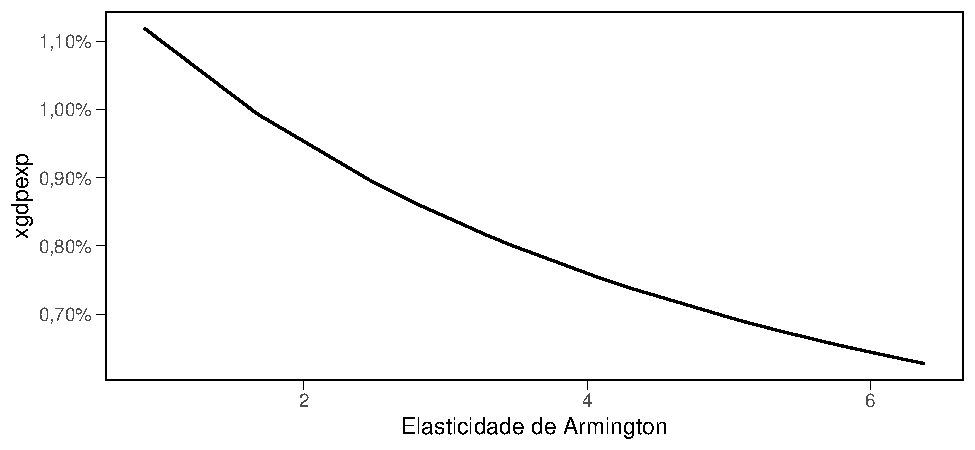
\includegraphics{minimal_files/figure-latex/unnamed-chunk-74-1.pdf}
\caption{Impacto \% no PIB para um aumento exógeno em 10\% na demanda
das famílias (X3TOT)\label{sensibilidade}}
\end{figure}

\hypertarget{experimento-2-aumento-do-saluxe1rio-real}{%
\subsubsection{Experimento 2: Aumento do salário
real}\label{experimento-2-aumento-do-saluxe1rio-real}}

No fechamento adotado, o salário real é definido exogenamente e o nível
de emprego torna-se endógeno. Assim, nesse segundo experimento,
verificamos quais seriam os impactos da elevação em 1\% do salário real.

Em primeiro lugar, precisamos definir novamente o objeto
\texttt{minimal}, uma vez que ele foi modificado no experimento
anterior.

\begin{Shaded}
\begin{Highlighting}[]
\NormalTok{minimal <-}\StringTok{ }\KeywordTok{list}\NormalTok{(}
  \DataTypeTok{sets =}\NormalTok{ sets,}
  \DataTypeTok{params =}\NormalTok{ params,}
  \DataTypeTok{variables =}\NormalTok{ variables,}
  \DataTypeTok{equations =}\NormalTok{ equations,}
  \DataTypeTok{update_equations =}\NormalTok{ update_equations}
\NormalTok{)}
\end{Highlighting}
\end{Shaded}

O segundo passo é definir o choque:

\begin{Shaded}
\begin{Highlighting}[]
\NormalTok{minimal}\OperatorTok{$}\NormalTok{params}\OperatorTok{$}\NormalTok{RW}\OperatorTok{$}\NormalTok{value[] <-}\StringTok{ }\FloatTok{1.01}
\end{Highlighting}
\end{Shaded}

Finalmente, iremos resolver o modelo novamente:

\begin{Shaded}
\begin{Highlighting}[]
\NormalTok{sol1 <-}\StringTok{ }\KeywordTok{solve_emr}\NormalTok{(minimal)}

\NormalTok{sol1}\OperatorTok{$}\NormalTok{sol}\OperatorTok{$}\NormalTok{message}
\end{Highlighting}
\end{Shaded}

\begin{verbatim}
## [1] "Successful convergence"
\end{verbatim}

\begin{table}[!h]

\caption{\label{tab:unnamed-chunk-78}Resultados da Simulação - Experimento 2}
\centering
\begin{tabular}[t]{lr}
\toprule
Variável & Variação \%\\
\midrule
Variação no emprego total (l) & -0,89\\
Variação no PIB nominal pela ótica do dispêndio (wgdpexp) & 0,54\\
Variação no PIB nominal (wgdpinc) & 0,54\\
Variação no deflator do PIB (pgdpexp) & 1,15\\
Variação no PIB real (xgdpexp) & -0,61\\
Balança comercial como razão do PIB (delB) & -0,51\\
Variação no índice de preços das famílias (p3tot) & 0,94\\
Variação da renda nominal das famílias (w3tot) & 0,94\\
Variação no salário nominal (p1lab) & 1,95\\
Variação no índice de preço do investimento (p2tot) & 0,97\\
Variação no índice de volume da exportação (x4tot) & -3,06\\
Variação no índice de preços da exportação (p4tot) & 0,62\\
Variação no índice de volume da importação (x0cif) & 0,87\\
\bottomrule
\end{tabular}
\end{table}

Para esse experimento, como esperado, ocorre uma redução no nível de
emprego (-0,89\%). Além disso, encontra-se um efeito negativo no PIB
real (-0,61\%), queda das exportações (-3,09\%) e aumento das
importações (+0,88\%).

\hypertarget{considerauxe7uxf5es-finais}{%
\section{Considerações Finais}\label{considerauxe7uxf5es-finais}}

O objetivo desse documento foi apresentar a estrutura de para construção
de modelos de equilíbrio parcial e geral no R, além de exemplificar com
as simulações podem ser realizadas. Esses modelos podem ser bastante
úteis para avaliações \emph{ex ante} de políticas. Dessa forma,
possibilitar a sua implementação em ambientes \emph{open source} podem
ajudar no ensino e disseminação desses modelos.

\newpage

\bibliography{referencias.bib}

\end{document}
